\section{Assignment 4: Image Stitching}
\label{sec:assignment4}

% TODO:
% make sure all figures are referenced
% more descriptive captions for figs
% discuss/show problematic spots
% create own photos stitching
% cite SIFT
% preamble (don't start with a subsection)

The goal of the assignment is to combine multiple overlapping photos of a scene into an (ideally seamless) panorama.
In order to do that, first corresponding points in the overlap region between images have to be found. From these correlations a homography can be calculated to project one of the images onto the other. Finally the homographies between neighbouring images are combined to a global mapping, so each image can be projected onto its final place in the panorama image. To test our implementation, besides the two provided image sets, we used a set of photos we took ourselves, and -- as an example for artificially generated images --  screenshots from the computer game Doom. These additional image sets are shown in Figure~\ref{fig:a4:imagesets}.

\newlength \mywidth \setlength \mywidth {0.15\textwidth}
\begin{figure}[h]
	\centering
	\begin{tabular}{ccccc}
	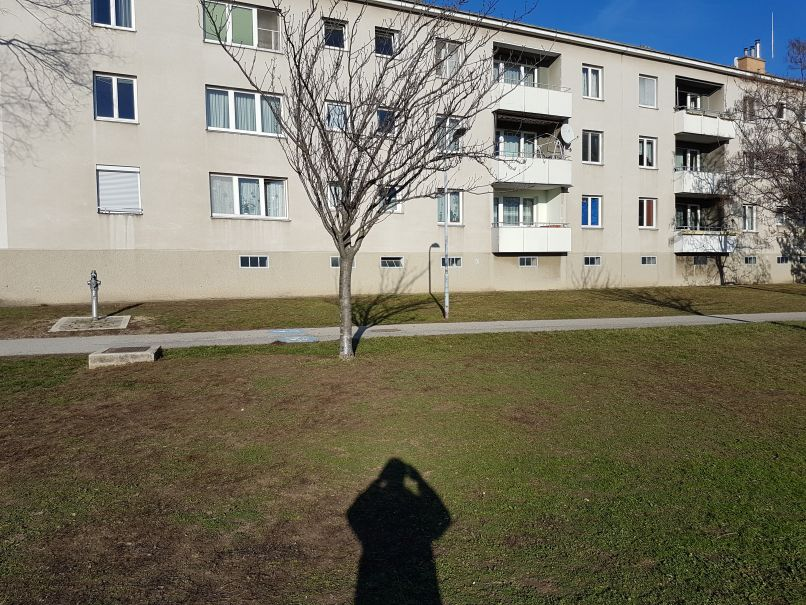
\includegraphics[width=\mywidth]{figures/seriesC_7.jpg} &
	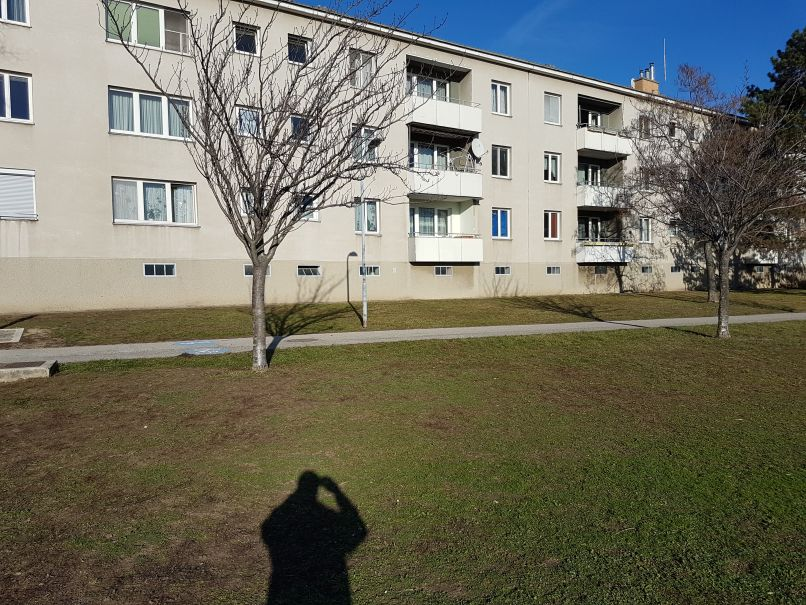
\includegraphics[width=\mywidth]{figures/seriesC_6.jpg} &
	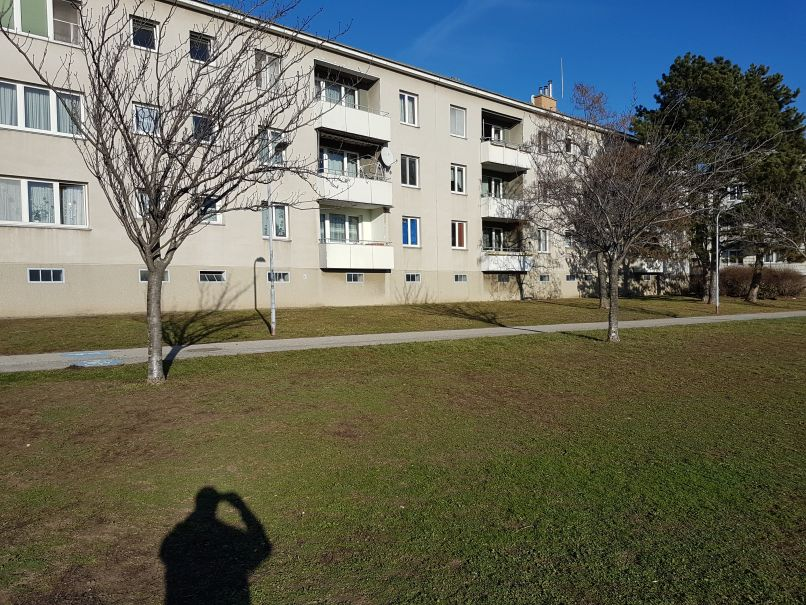
\includegraphics[width=\mywidth]{figures/seriesC_5.jpg} &
	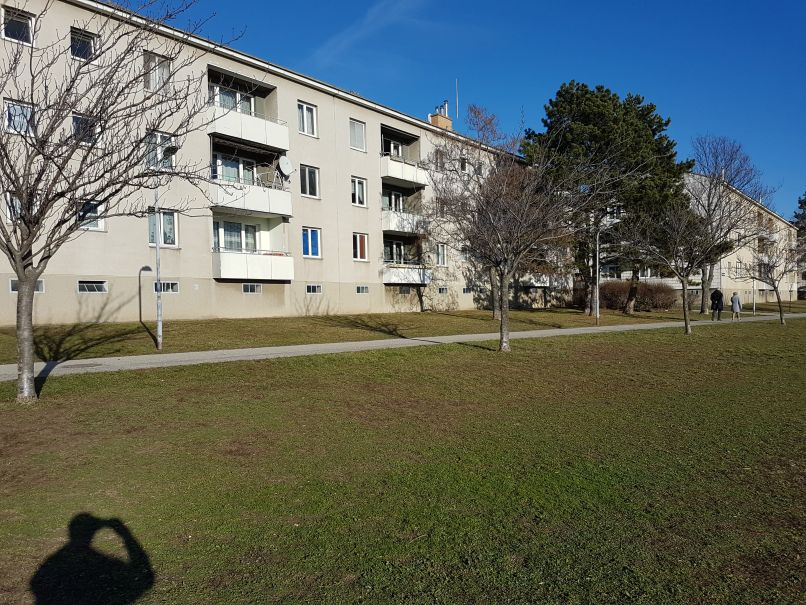
\includegraphics[width=\mywidth]{figures/seriesC_4.jpg} &
	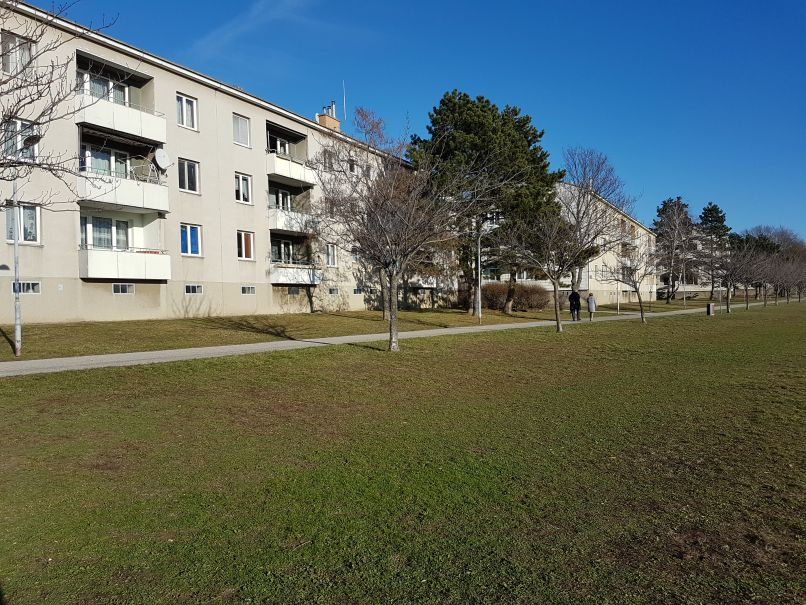
\includegraphics[width=\mywidth]{figures/seriesC_3.jpg} \\
	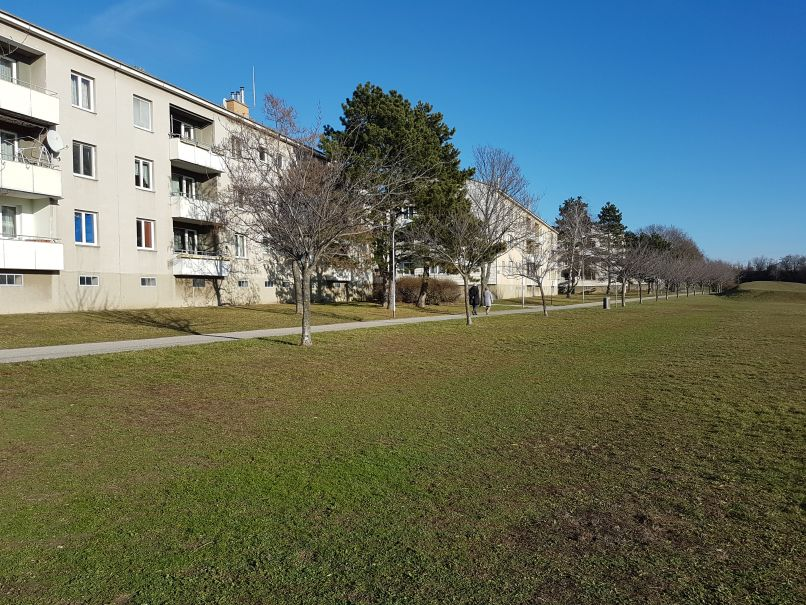
\includegraphics[width=\mywidth]{figures/seriesC_2.jpg} &
	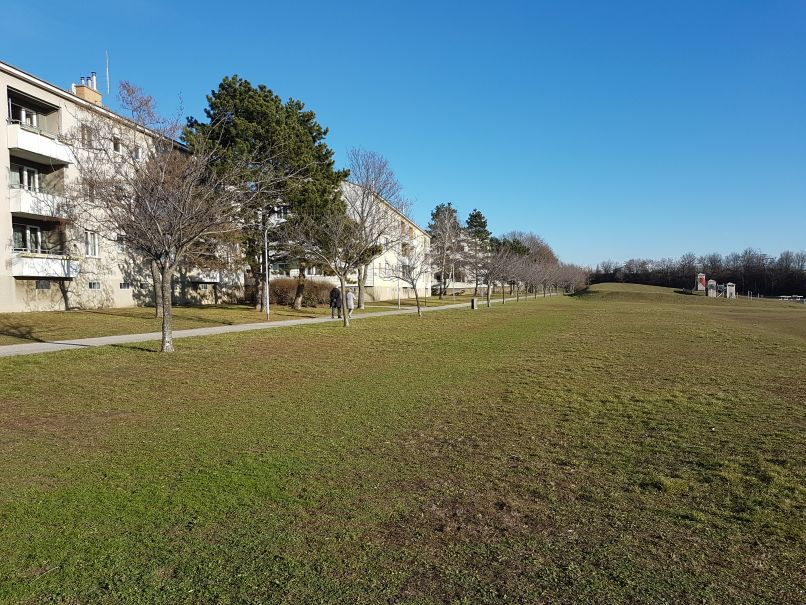
\includegraphics[width=\mywidth]{figures/seriesC_1.jpg} &
	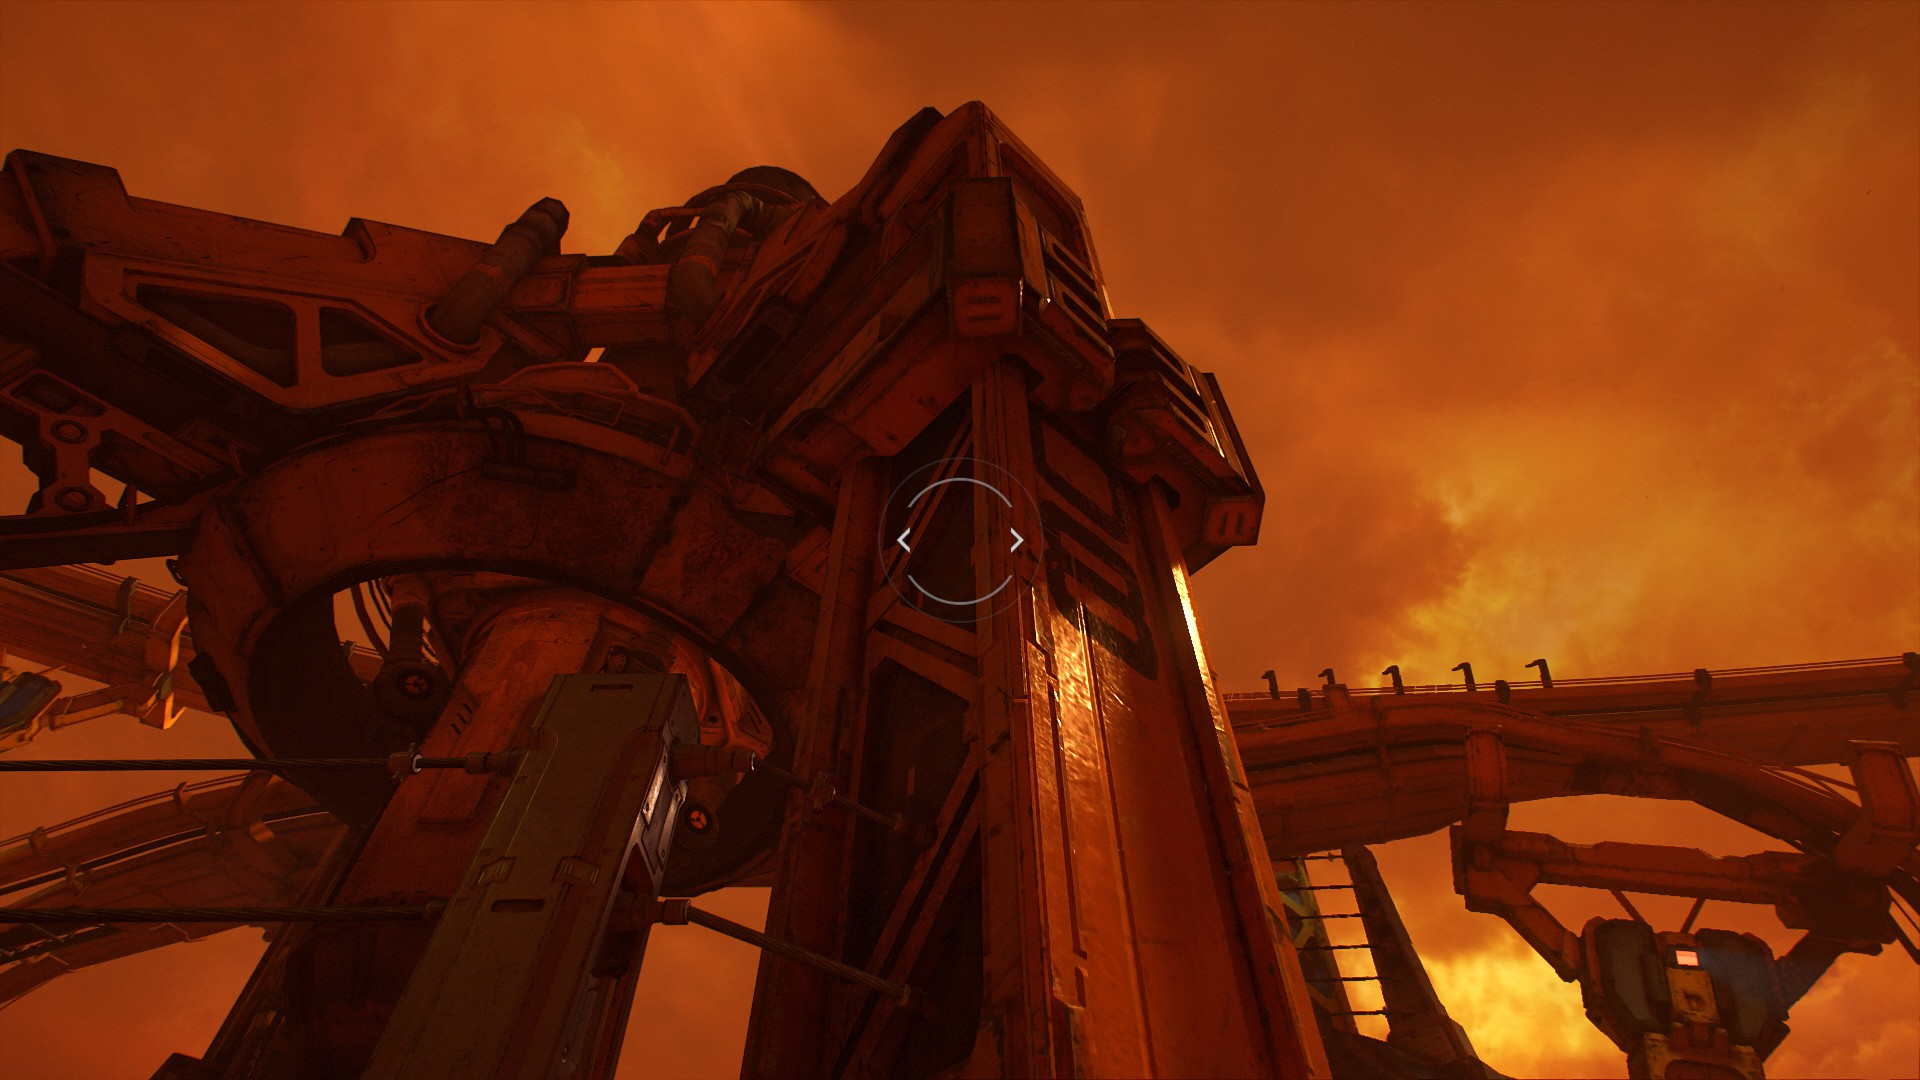
\includegraphics[width=\mywidth]{figures/doom1.jpg} &
	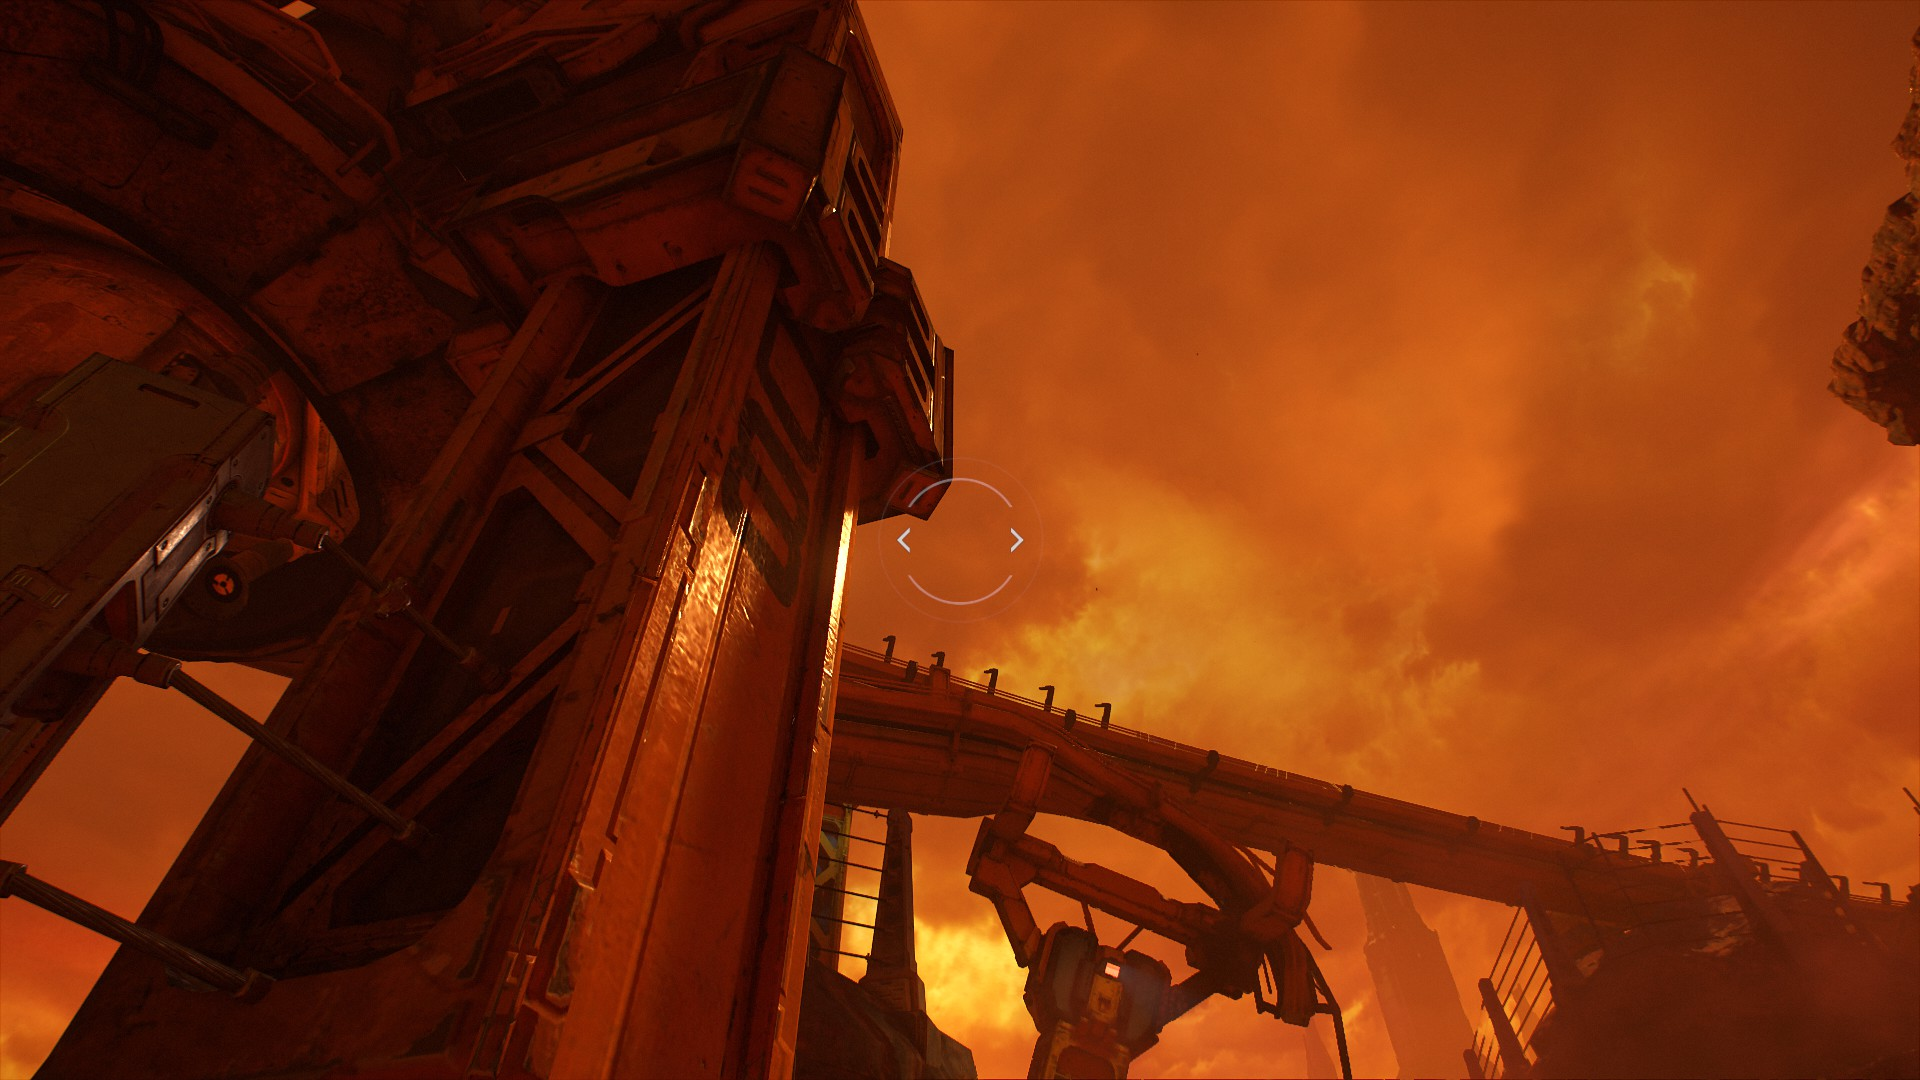
\includegraphics[width=\mywidth]{figures/doom2.jpg} &
	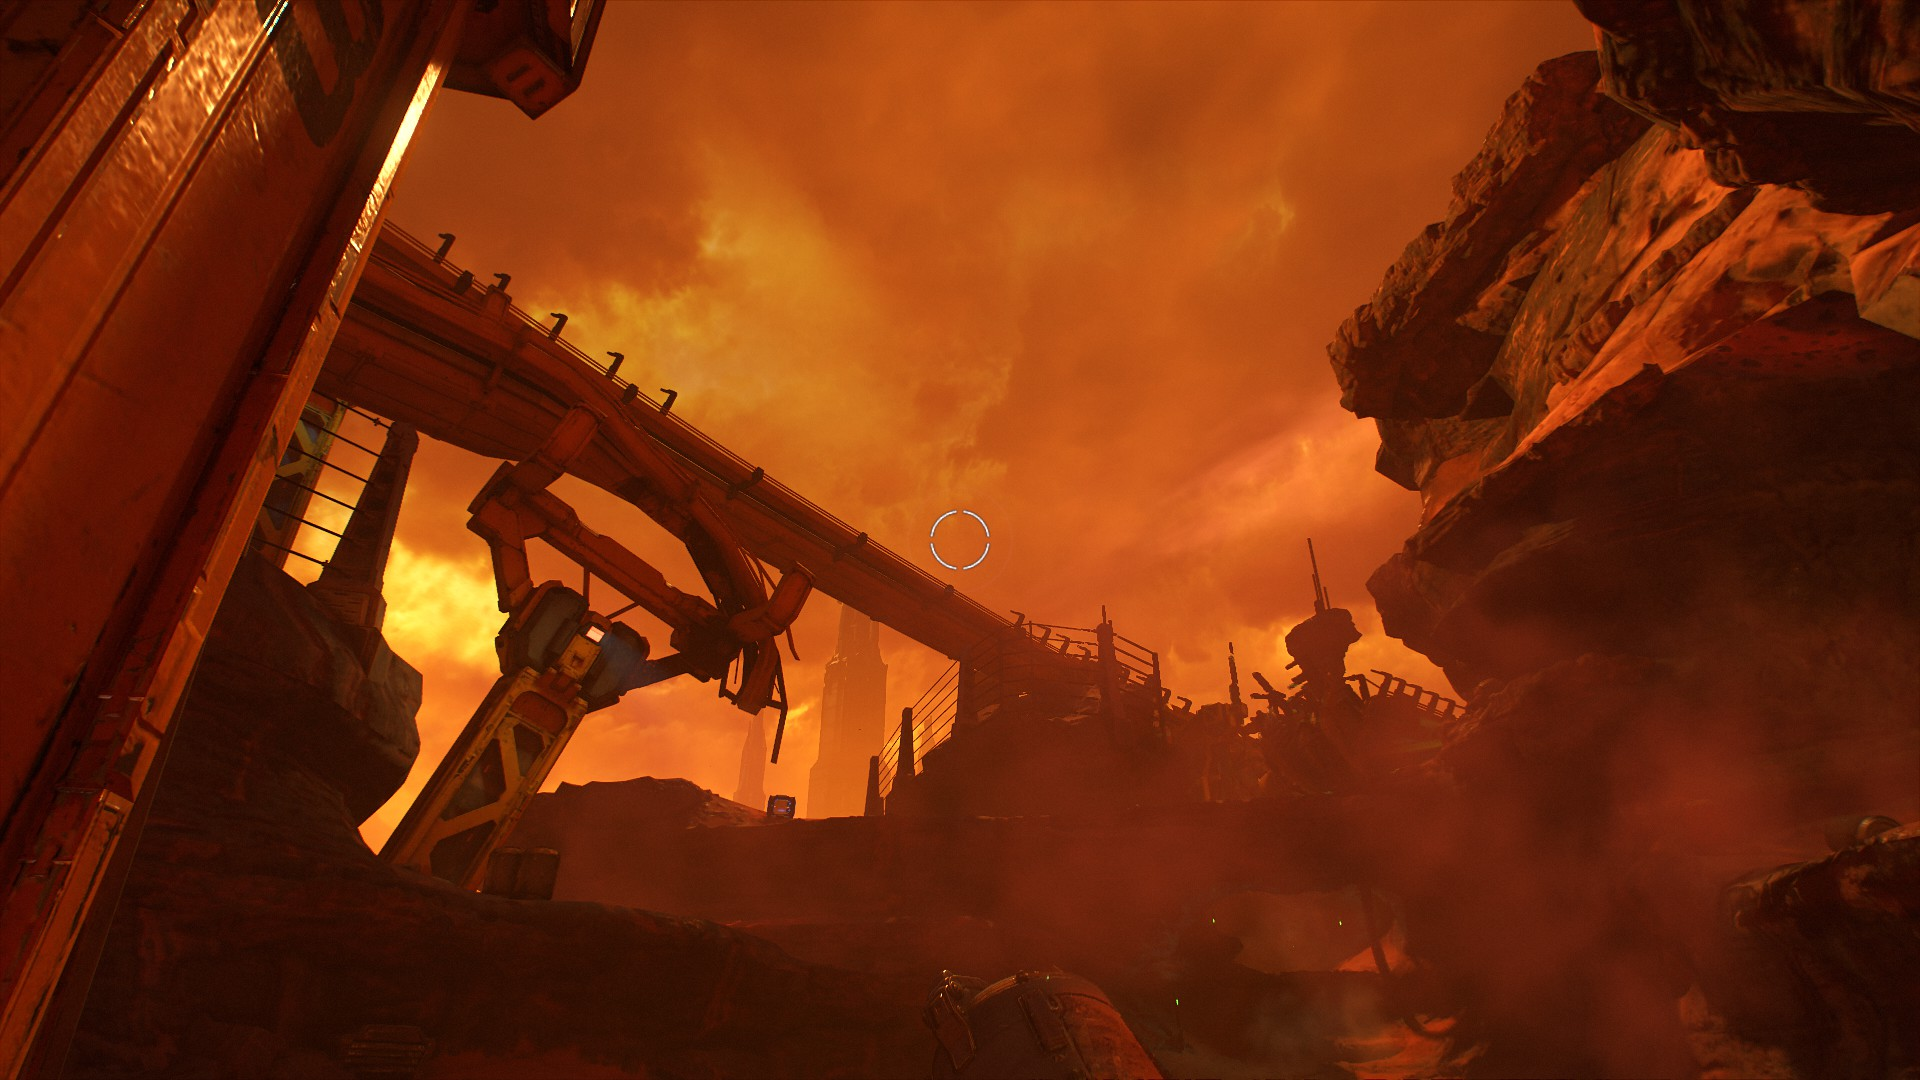
\includegraphics[width=\mywidth]{figures/doom3.jpg} \\

	\end{tabular}
	\caption{Additional image sets used for experimentation.}
	\label{fig:a4:imagesets}
\end{figure}

\subsection{SIFT Interest Point Detection}

In the first step we used the function \texttt{vl\_sift} to run the Scale Invariant Feature Transform (SIFT) \cite{Lowe04} algorithm for key point detection. As we did not need the key descriptors at this stage, we only acquired the position of each key point, along with its scale and orientation. SIFT uses Difference of Gaussians (DoG) to approximate the Logarithm of Gaussians (LoG): to examine different scales, the SIFT algorithm creates a minimum of five different Gaussian images per octave; the difference of these images (DoGs) are then used for maxima detection, similar to the blob detection algorithm from the previous assignment. 

To find the orientation of the key points, depending on the scale, a region around the key point center is chosen. The gradient magnitudes and orientations are calculated for each pixel in this region, and the result is placed in a histogram consisting of 36 bins (10$^\circ$ per bin). The largest bin of the histogram is the orientation of the key point; other bins very close to the maximum are converted into new key points (same position and scale, but with a different orientation). The key point orientation is important, because further calculations (descriptors) will be relative to this orientation, which ensures orientation invariance for matching key points.

The function \texttt{vl\_plotframe} illustrates the results. A circle's radius correspond to the scale of the associated key point and the line is its orientation as visualized in Figure \ref{fig:a4:vlplotframe}.

\begin{figure}[h]
	\centering
	\begin{tabular}{cc}
	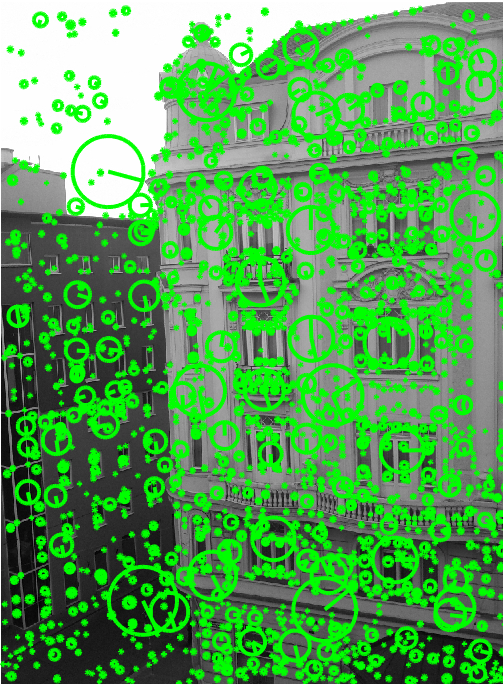
\includegraphics[width=0.4\textwidth]{figures/vl_plotframe_officeview1.png} &
	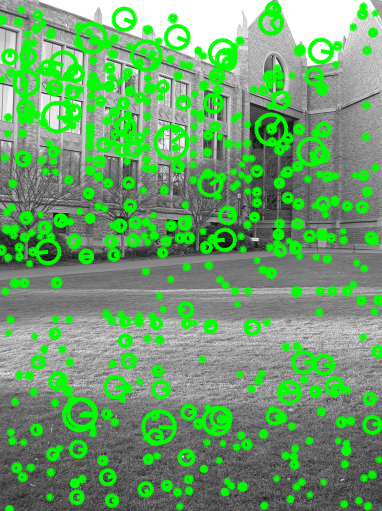
\includegraphics[width=0.4\textwidth]{figures/vl_plotframe_campus4.png} 

	\end{tabular}
	\caption{SIFT key point detection: scale and orientation of key points.}
	\label{fig:a4:vlplotframe}
\end{figure}

\subsection{Interest Point Matching and Image Registration}

Similar to the previous task, first we extracted all key points via SIFT, this time along with the associated descriptor of each key point. The descriptors are an array of 128 numbers constructed as follows: First the 16x16 window around the key point is broken down into smaller 4x4 windows. Within each of the 16 windows the gradients are calculated and subsequently put into an 8 bin histogram (45$^\circ$ each). The magnitude contributed by each gradient also depends on the distance from the key point (using Gaussian weights). 

Each of the 128 resulting numbers is normalized and reduced by the key point's orientation (to ensure orientation invariance) and subsequently clamped at 0.2 (to ensure illumination invariance) before being normalized to a unit vector again.

%\begin{figure}[h]
%	\centering
%	\begin{tabular}{cc}
%	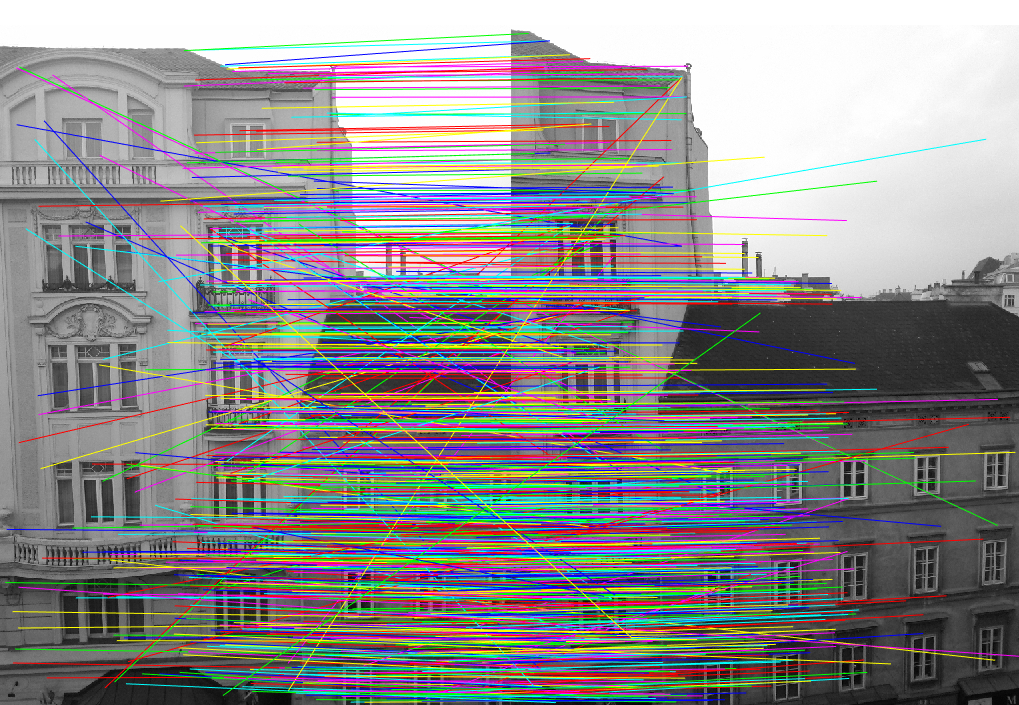
\includegraphics[width=0.45\textwidth]{figures/vl_ubcmatch1.png} &
%	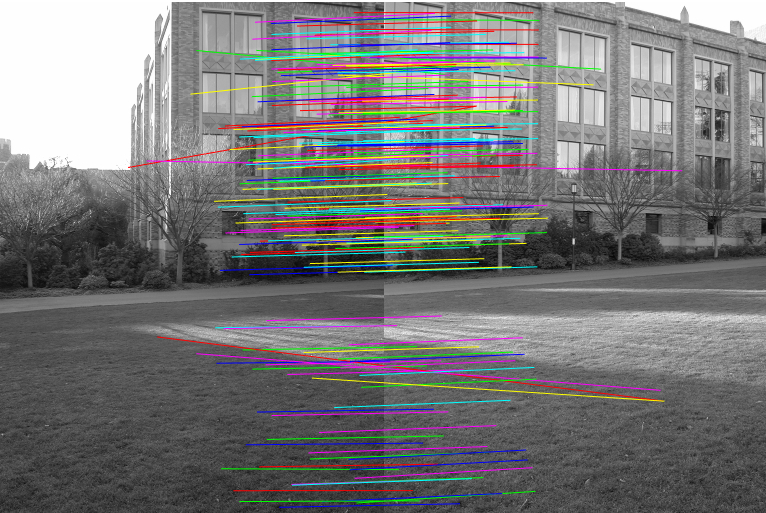
\includegraphics[width=0.45\textwidth]{figures/vl_ubcmatch2.png} 
%
%	\end{tabular}
%	\caption{The resuts of \texttt{vl\_ubcmatch}. }
%	\label{fig:a4:ubcmatch}
%\end{figure}

\texttt{vl\_ubcmatch} is used as a first, basic, matching step. For each descriptor in the first image, \texttt{vl\_ubc\-match} attempts to find the closest descriptor in the target image using the L2 norm\footnote{Least squares, Euclidean norm} of the difference between the two. This basic algorithm may return many false positive matches though. The result is illustrated in the top row of Figure \ref{fig:a4:matching}.

To eliminate potential false positive matches, a RANdom SAmple Consensus (RANSAC) \cite{Fischler81} scheme is applied: Basically, a homography is estimated by using 4 random sample matches out of all matches found by \texttt{vl\_ubcmatch}, which is then applied to all other key points via \texttt{transformPointsforward}. The number of inliers, i.e.,  those matches having their Euclidean distance smaller than a certain threshold $T$, is determined and remembered.
%The RANSAC algorithm is applied N times and the homography with the largest number of inliers is returned as the correct estimation.
This procedure is repeated $N$ times, and finally only the inliers of the best homography found (i.e., the one yielding the highest number of inliers) are used to estimate the final homography estimation.
Figure \ref{fig:a4:matching} shows the remaining (inlier) matches after running RANSAC in the middle row, and the false positive matches eliminated in the bottom row.

\setlength \mywidth {0.47\textwidth}
\begin{figure}[h]
	\centering
	\begin{tabular}{cc}
	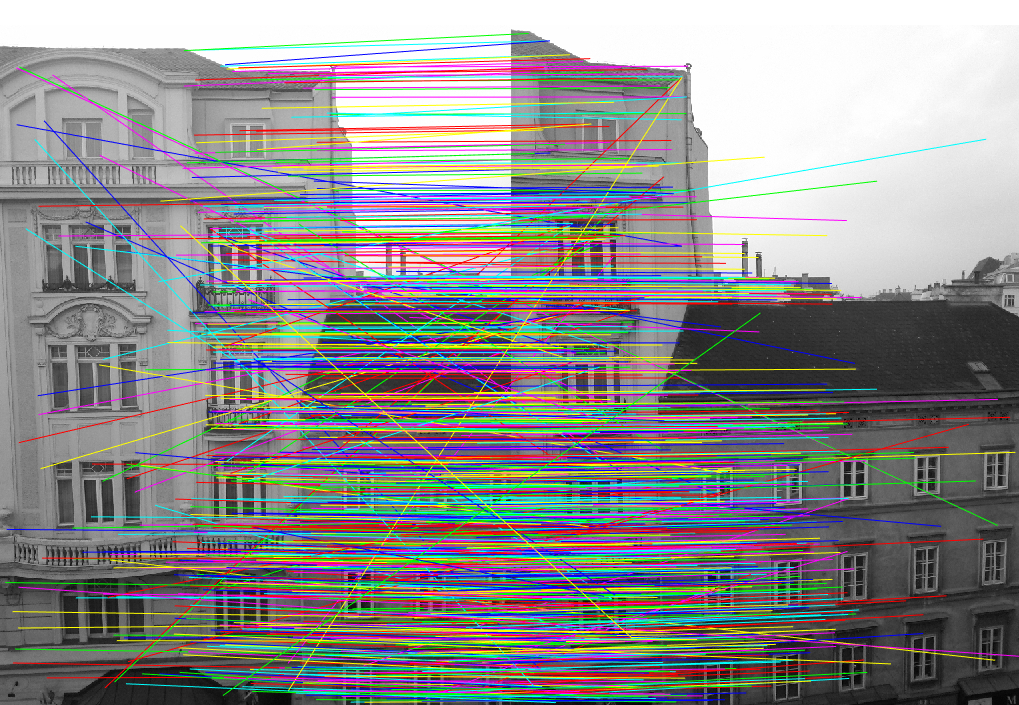
\includegraphics[width=\mywidth]{figures/vl_ubcmatch1.png} &
	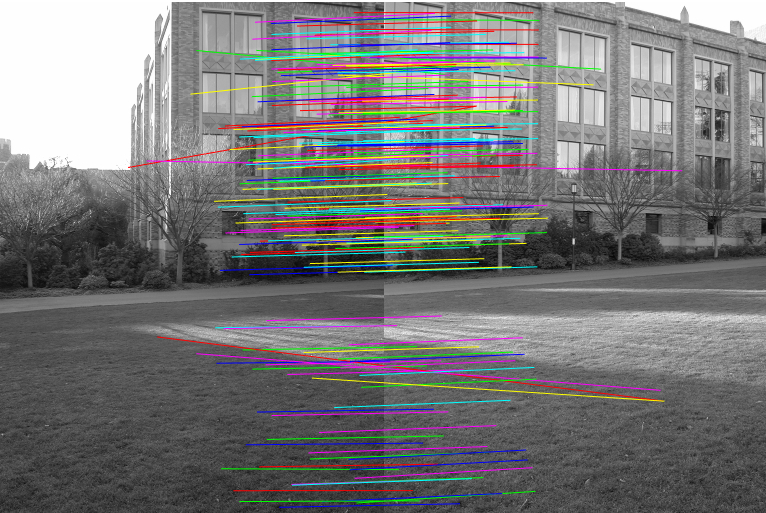
\includegraphics[width=\mywidth]{figures/vl_ubcmatch2.png} \\
	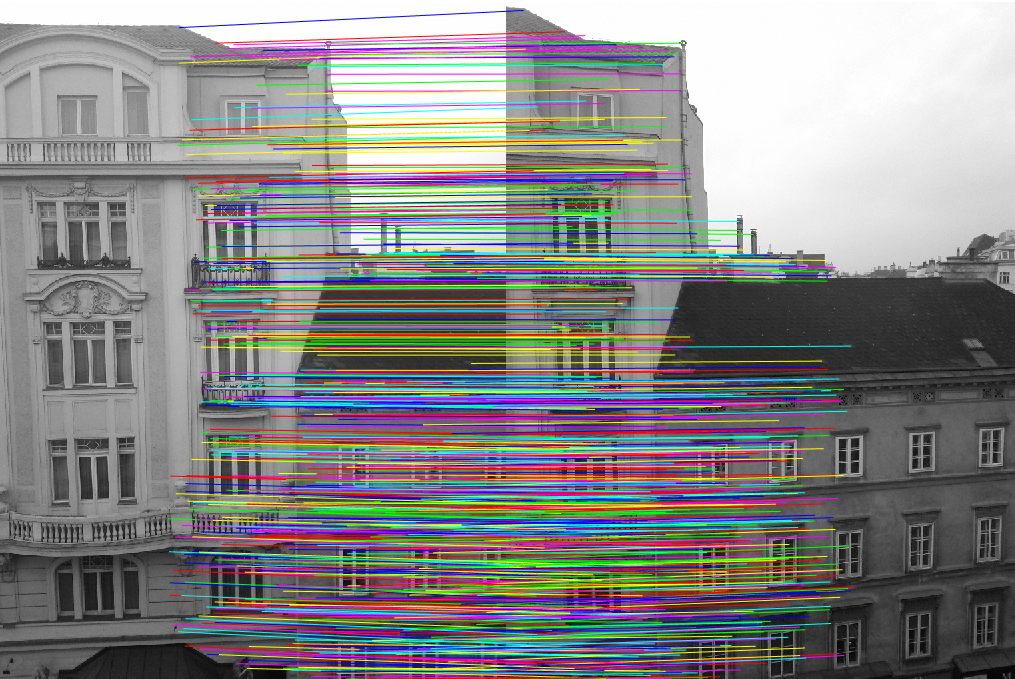
\includegraphics[width=\mywidth]{figures/ransac1.png} &
	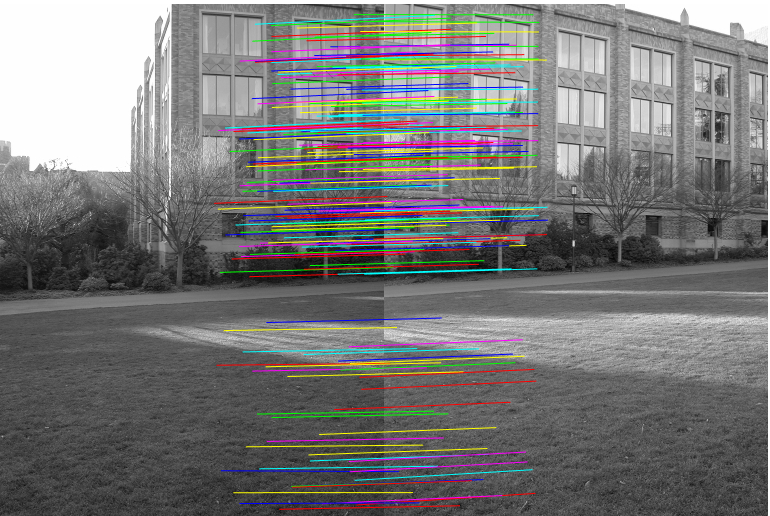
\includegraphics[width=\mywidth]{figures/ransac2.png} \\
	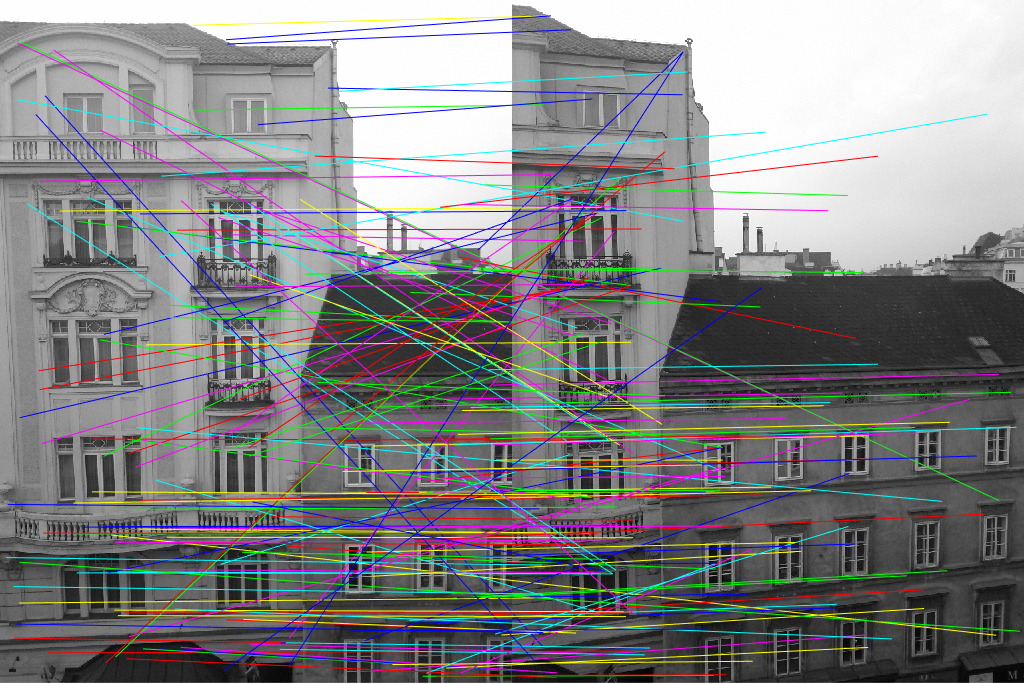
\includegraphics[width=\mywidth]{figures/ransac_removes1.png} &
	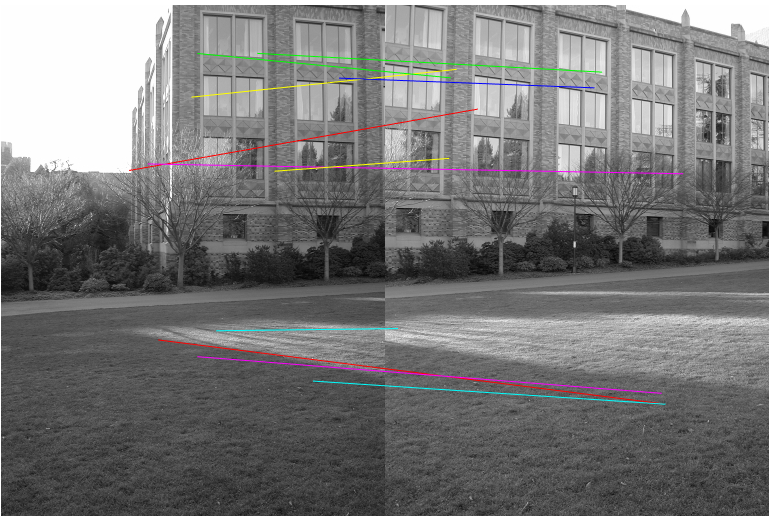
\includegraphics[width=\mywidth]{figures/ransac_removes2.png} \\

	\end{tabular}
	\caption{Top: Initial matchings obtained by \texttt{vl\_ubcmatch}. Middle: Correct matches (inliers determined by RANSAC). Bottom: False matches (outliers removed by RANSAC).}
	\label{fig:a4:matching}
\end{figure}

%\begin{figure}[h]
%	\centering
%	\begin{tabular}{cc}
%	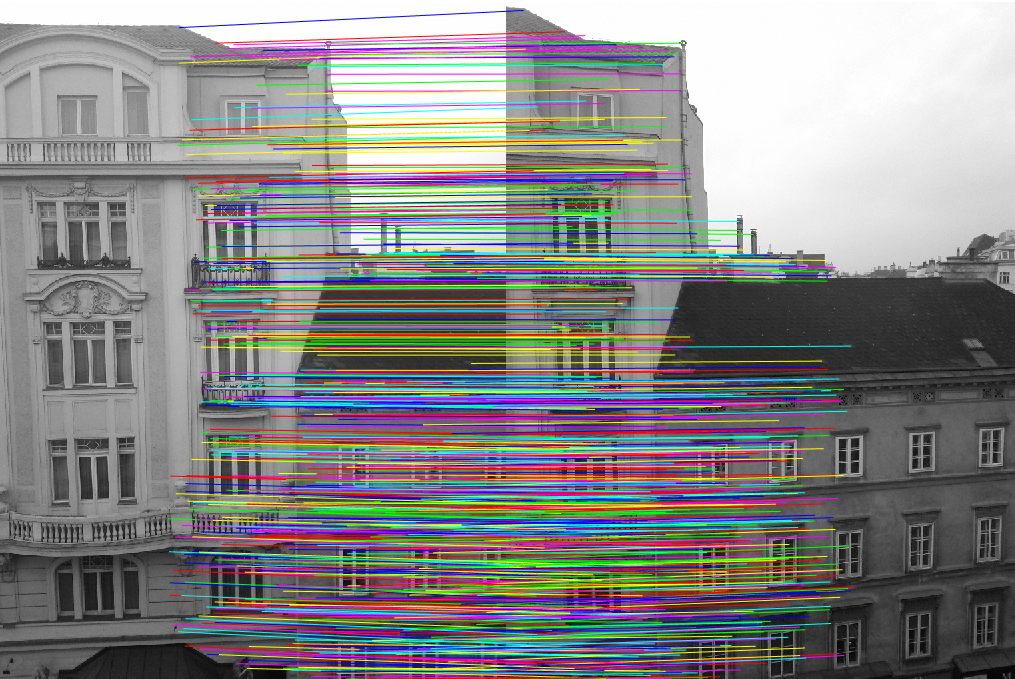
\includegraphics[width=0.45\textwidth]{figures/ransac1.png} &
%	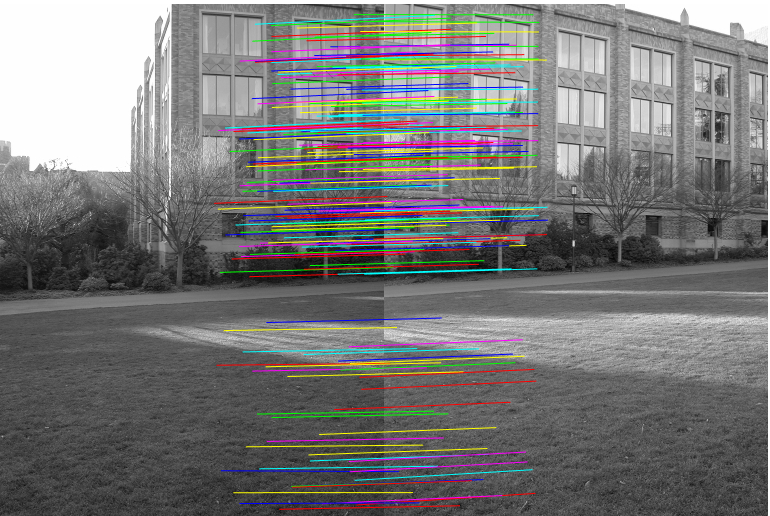
\includegraphics[width=0.45\textwidth]{figures/ransac2.png} 
%
%	\end{tabular}
%	\caption{The matched key points after applying RANSAC. }
%	\label{fig:a4:ransac}
%\end{figure}
%
%\begin{figure}[h]
%	\centering
%	\begin{tabular}{cc}
%	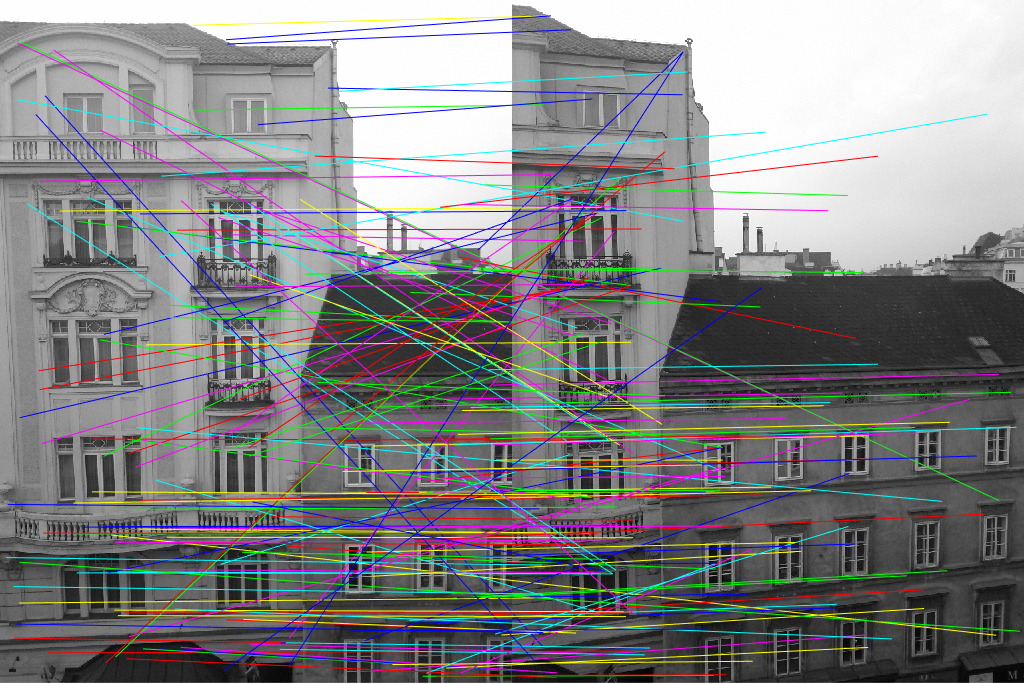
\includegraphics[width=0.45\textwidth]{figures/ransac_removes1.png} &
%	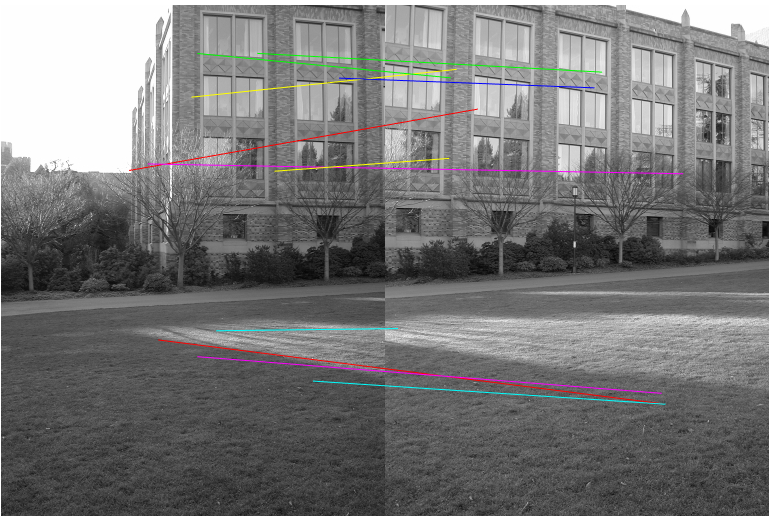
\includegraphics[width=0.45\textwidth]{figures/ransac_removes2.png} 
%
%	\end{tabular}
%	\caption{Potentially false matches estimated by \texttt{vl\_ubcmatch} and removed by RANSAC.}
%	\label{fig:a4:ransac_removes}
%\end{figure}


\setlength \mywidth {0.33\textwidth}
\begin{figure}[h]
	\centering
	\begin{tabular}{cc}
	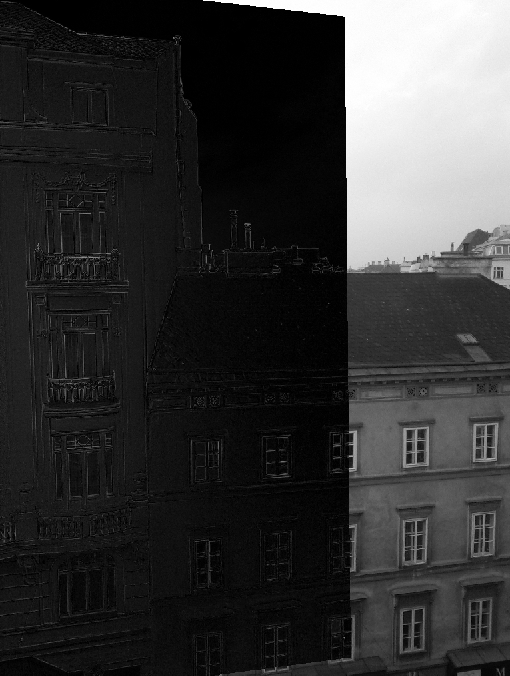
\includegraphics[width=\mywidth]{figures/diff1.png} &
	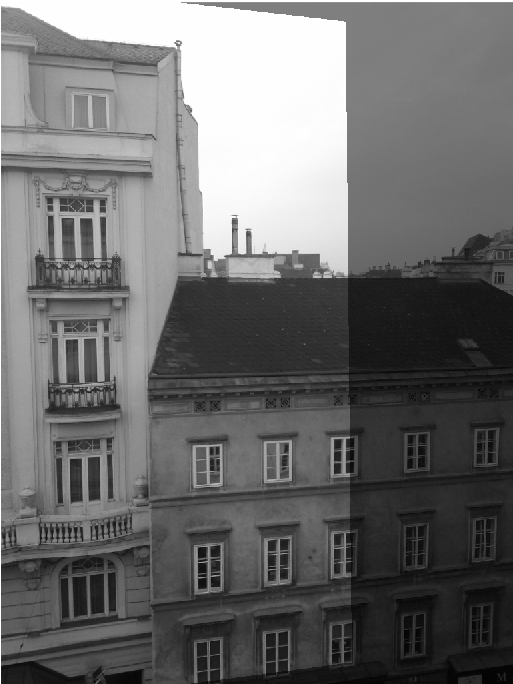
\includegraphics[width=\mywidth]{figures/overlay1.png} \\
	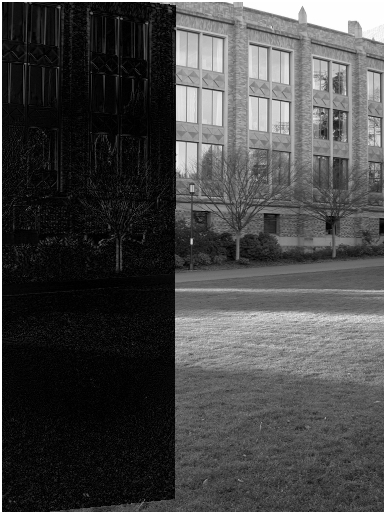
\includegraphics[width=\mywidth]{figures/diff2.png} &
	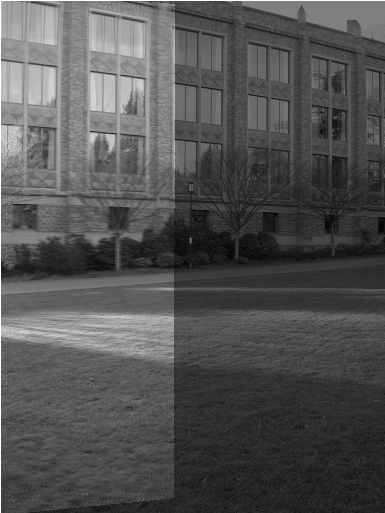
\includegraphics[width=\mywidth]{figures/overlay2.png} 

	\end{tabular}
	\caption{Difference (left side, dark areas) and overlay (right) view of aligned images.}
	\label{fig:a4:diffs}
\end{figure}


After applying the above steps the images are considered well aligned. Figure \ref{fig:a4:diffs} shows absolute differences and overlays of pairs of matched images, using the estimated homography.



\begin{figure}[h]
	\centering
	\begin{tabular}{cc}
	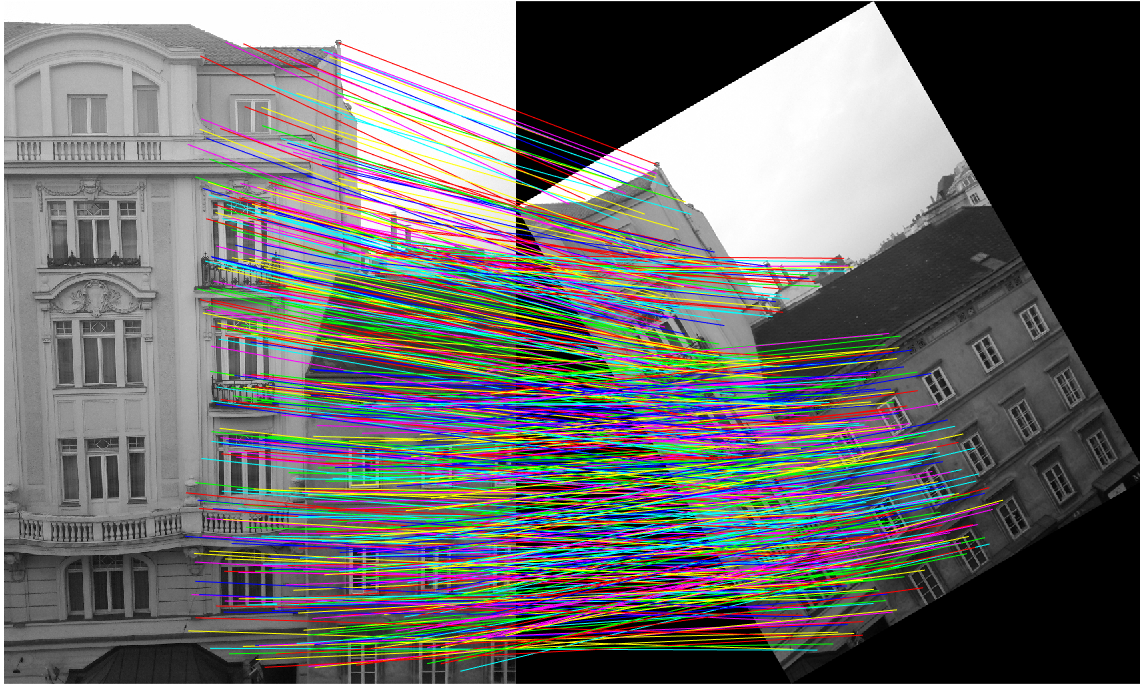
\includegraphics[width=0.59\textwidth]{figures/rotation_ransac.png} &
	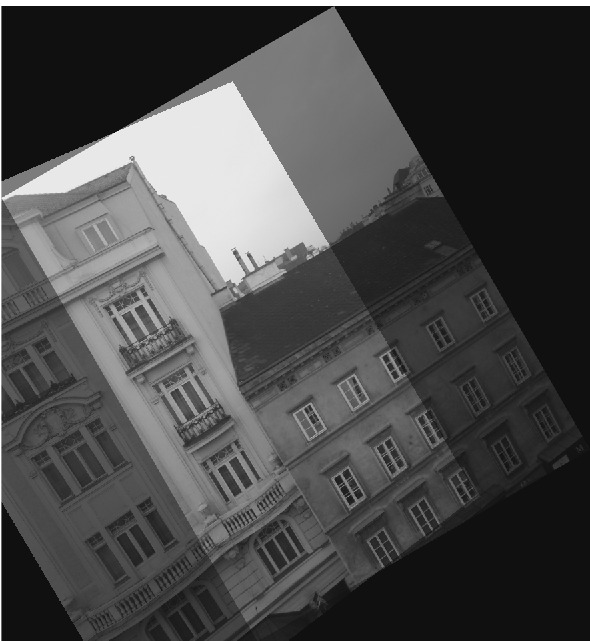
\includegraphics[width=0.33\textwidth]{figures/rotation_overlay.png} 

	\end{tabular}
	\caption{Post RANSAC matches after rotating and rescaling and the aligned result.}
	\label{fig:a4:rotationscale}
\end{figure}

As described above, in a key point descriptor the gradient orientation of each pixel is adjusted to the key point's dominant orientation before being added to the associated histogram. Therefore the results should be invariant to changes in image rotation. Additionally the SIFT algorithm is also scale invariant as described in the first section. That this is indeed the case can be seen in Figure \ref{fig:a4:rotationscale}, where one of the images has been rescaled and rotated.

\FloatBarrier % keep figures above!

\subsection{Image Stitching}

To stitch images together for the purpose of creating a panorama view, first the homography is estimated between each pair of adjacent images. One image is selected as reference image (usually the one in the centre of the panorama) and, utilizing the homographies estimated before, the homography of each image to the reference image is calculated. From this complete set of homographies, the final size of the panorama is calculated, and each image then is projected onto its correct place within the panorama. The results of independently projecting the images is shown in Figure~\ref{fig:a4:noblend}.

\begin{figure}[h]
	\centering
	\begin{tabular}{cc}
	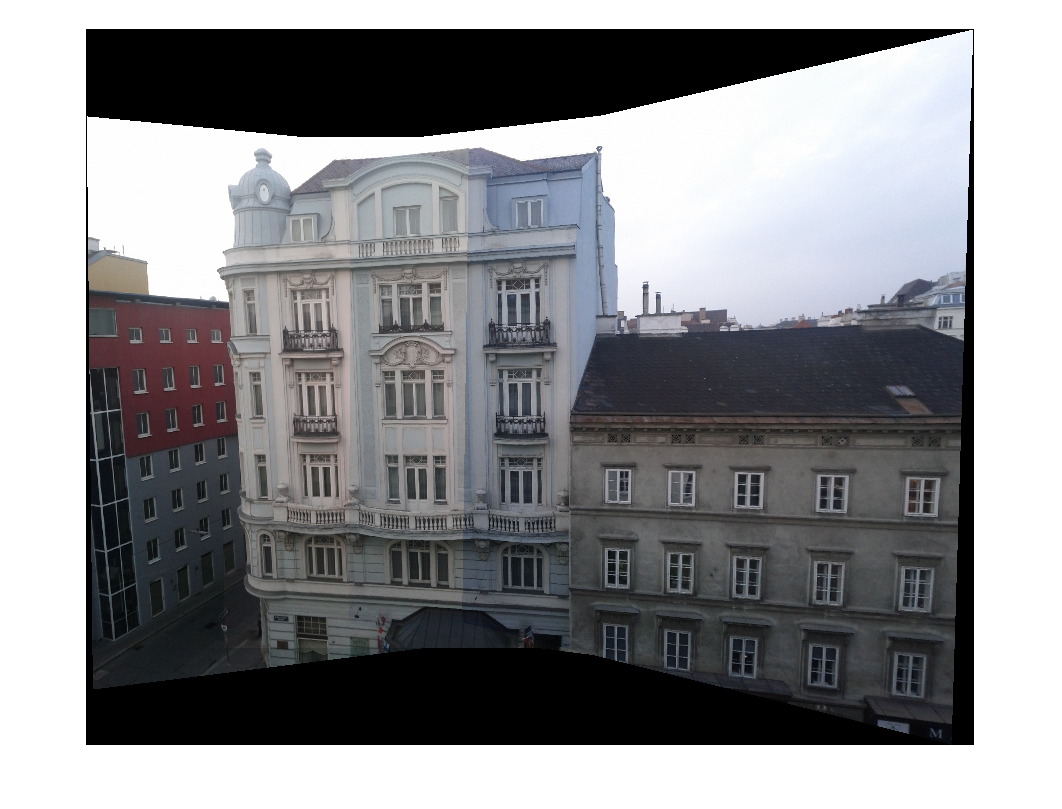
\includegraphics[width=0.45\textwidth]{figures/office_p_b.png} &
	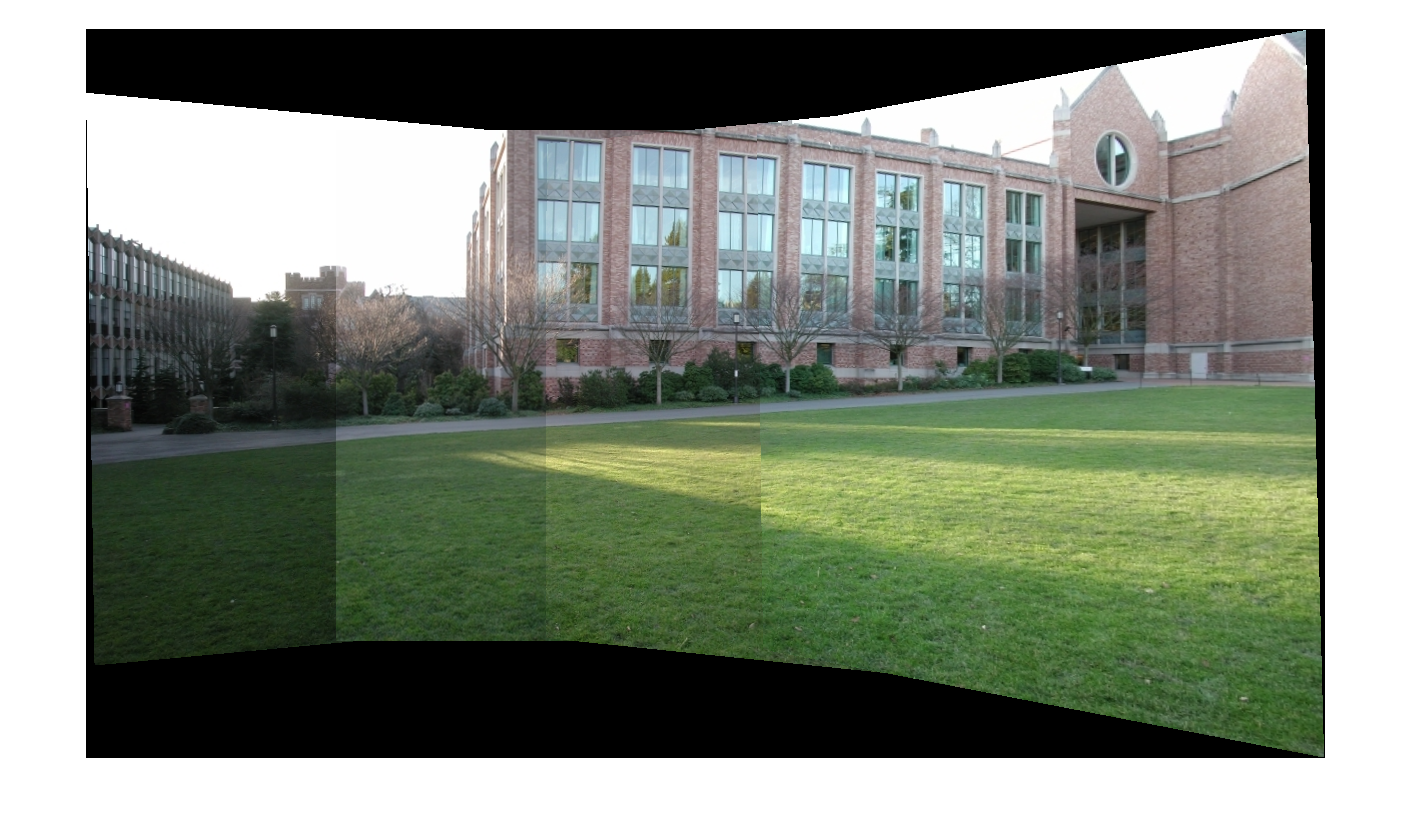
\includegraphics[width=0.45\textwidth]{figures/campus_p_b.png} \\
	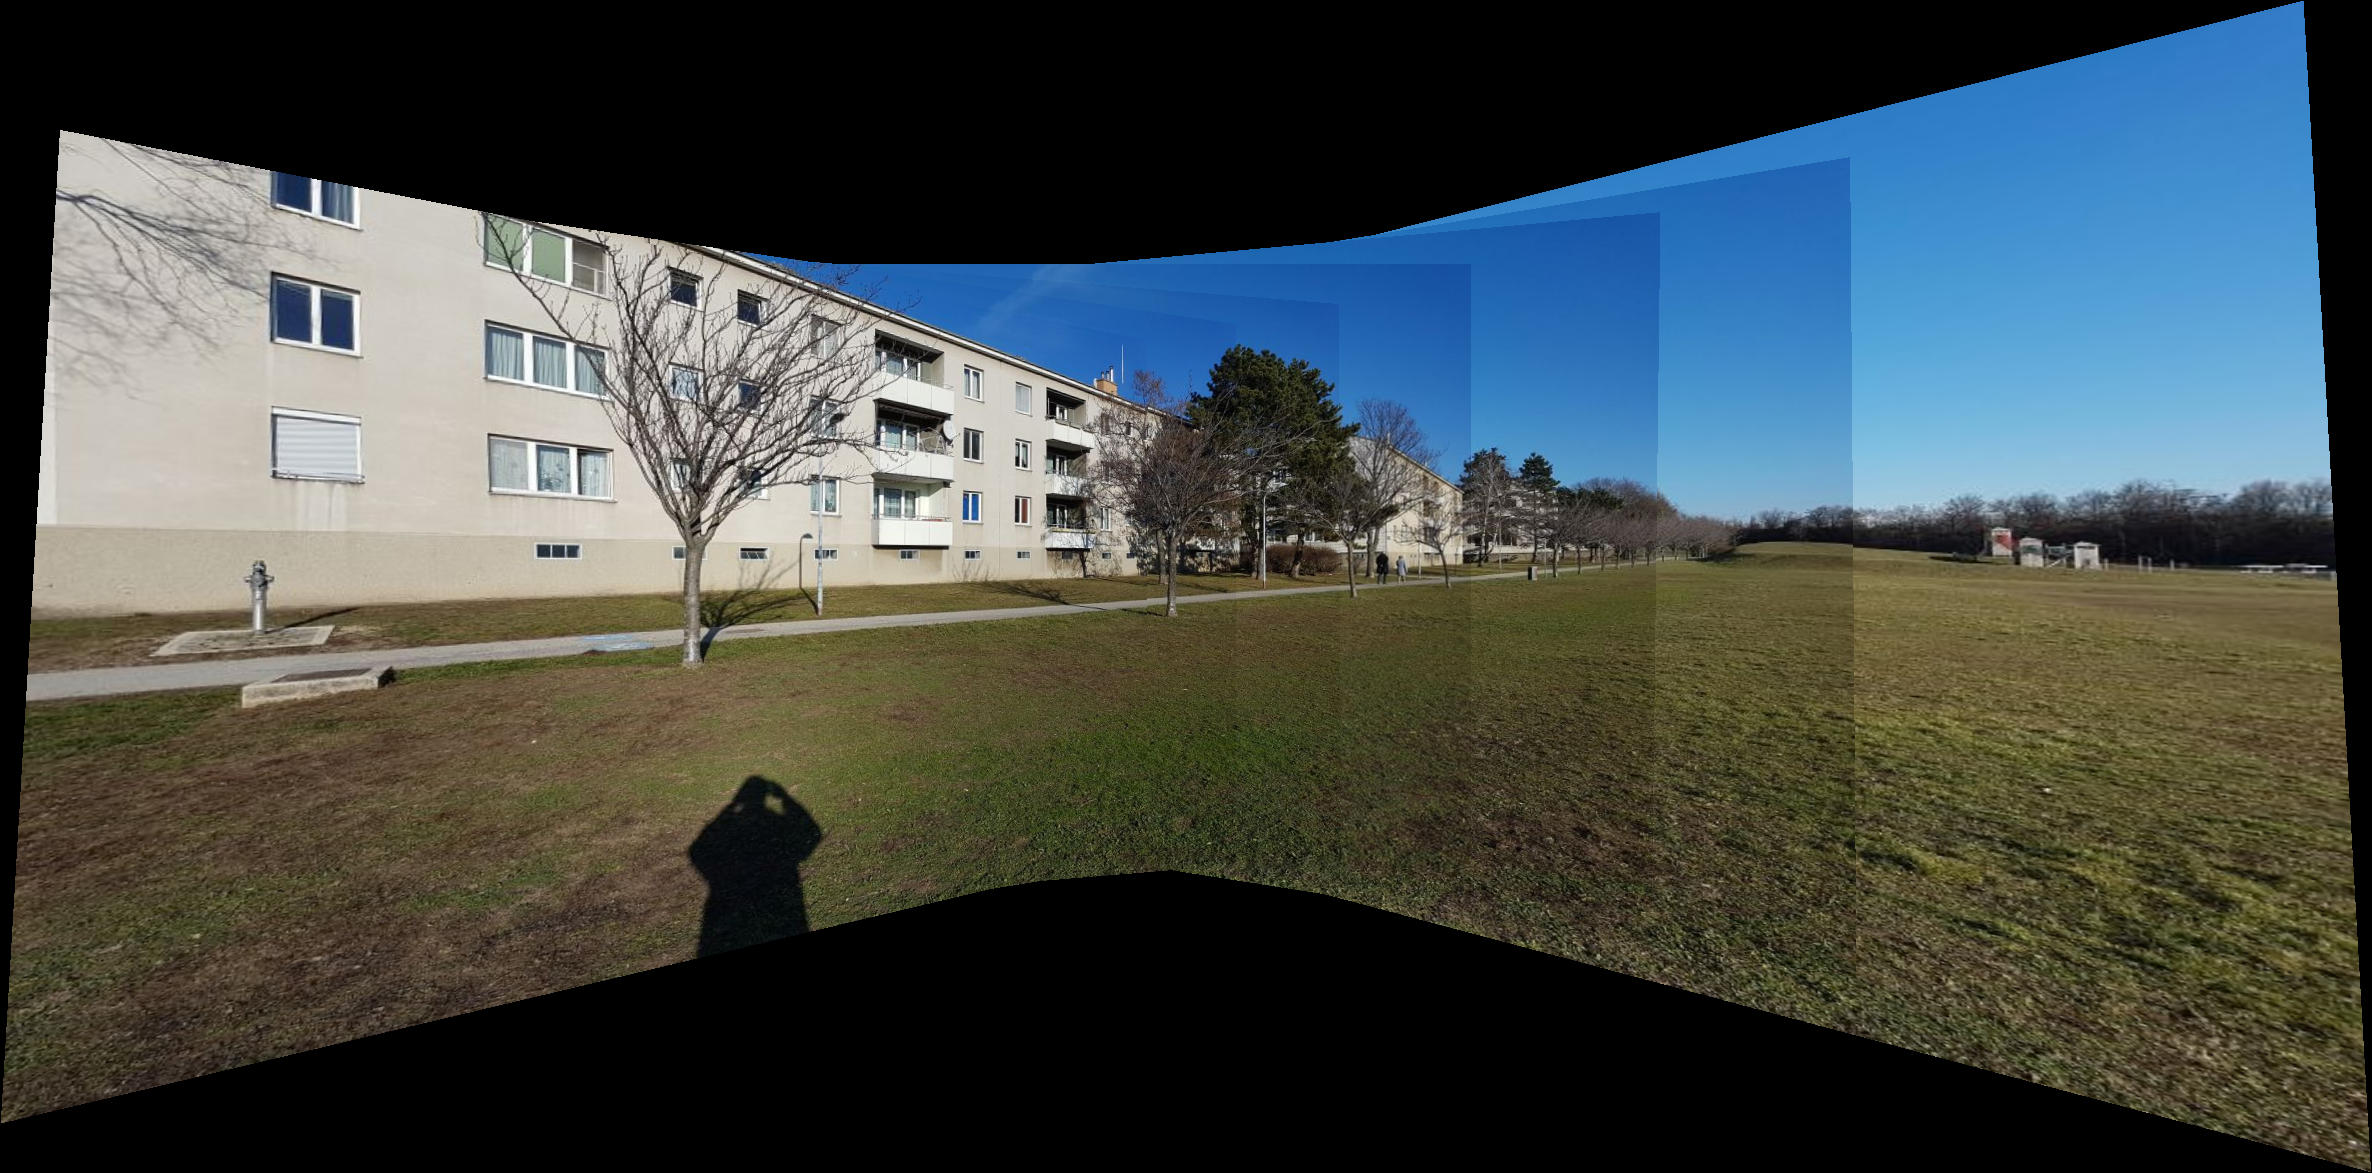
\includegraphics[width=0.45\textwidth]{figures/own_p_b.png} &
	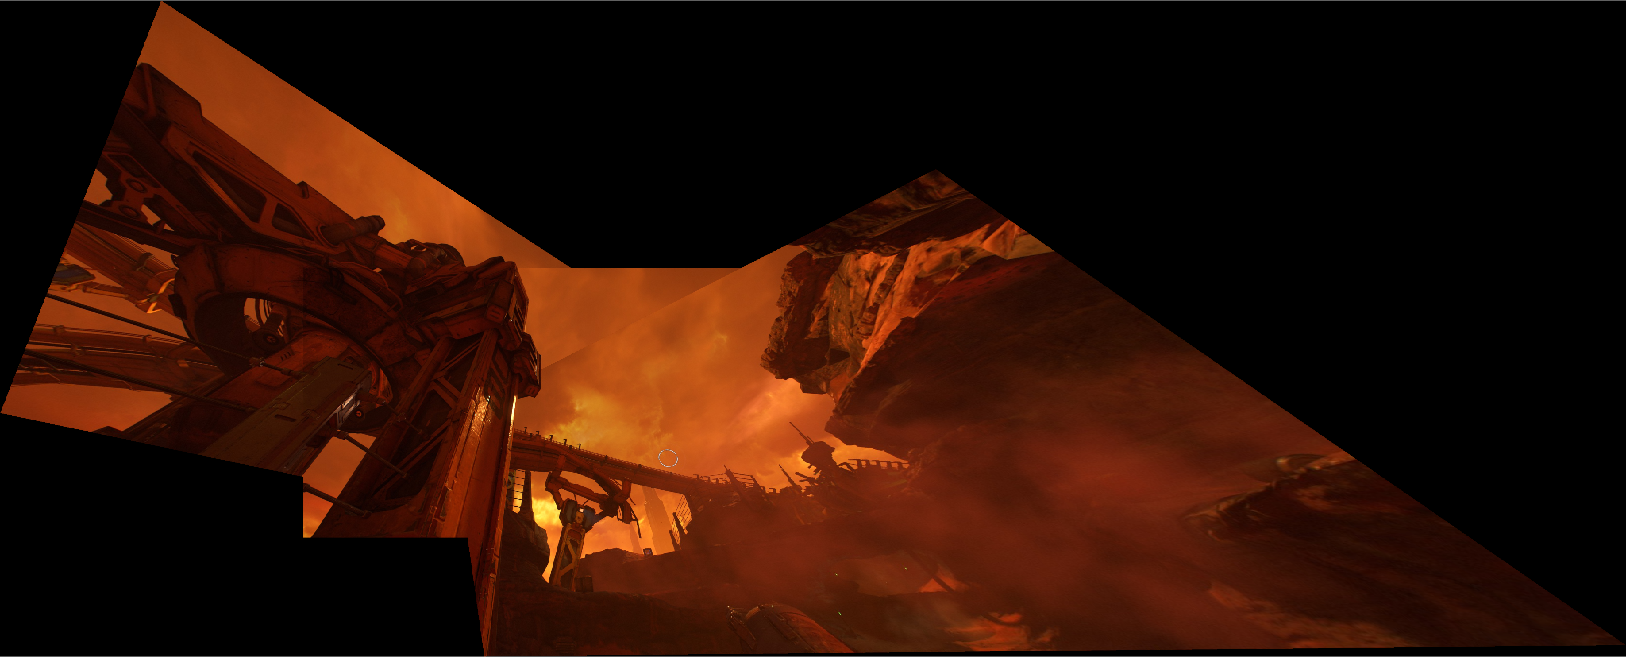
\includegraphics[width=0.45\textwidth]{figures/doom_p_b.png}

	\end{tabular}
	\caption{Resulting panorama images without blending.}
	\label{fig:a4:noblend}
\end{figure}

%The panorama images shown in figures \ref{fig:a4:pano1} and \ref{fig:a4:pano2} use feathering to blend the images together. Would we use no blending, the final panorama image would look quite different as illustrated by Figure \ref{fig:a4:noblend}.
However, just overlaying the images results in clearly visible seams, due to different brightness. In order to create a seamless panorama, a feathering technique is used: the basic idea is, that the centre values of each image are more important than its border values. For this purpose, we calculated a normalised distance-to-border map for each image, using MATLAB's \texttt{bwdist} function (a kind of $\alpha$-channel), representing the relative importance of each image pixel. When projecting the images to the panorama, this mask is also projected with the same homography, and the final color for each pixel is calculated as a weighted sum of the image contributions, the weight being the relation of each image's alpha value to the sum of alpha values for this pixel:
$$ O(x,y)=\frac{\sum_{i=1}^{n}{(R_i,G_i,B_i) \alpha_i}}{\sum_{i=1}^{n}{\alpha_i}} $$
The result of this procedure is that the overlapping regions are smoothly blended between the contributing images, as demonstrated in Figure~\ref{fig:a4:feathering}.

\begin{figure}[h]
	\centering
	\begin{tabular}{cc}
	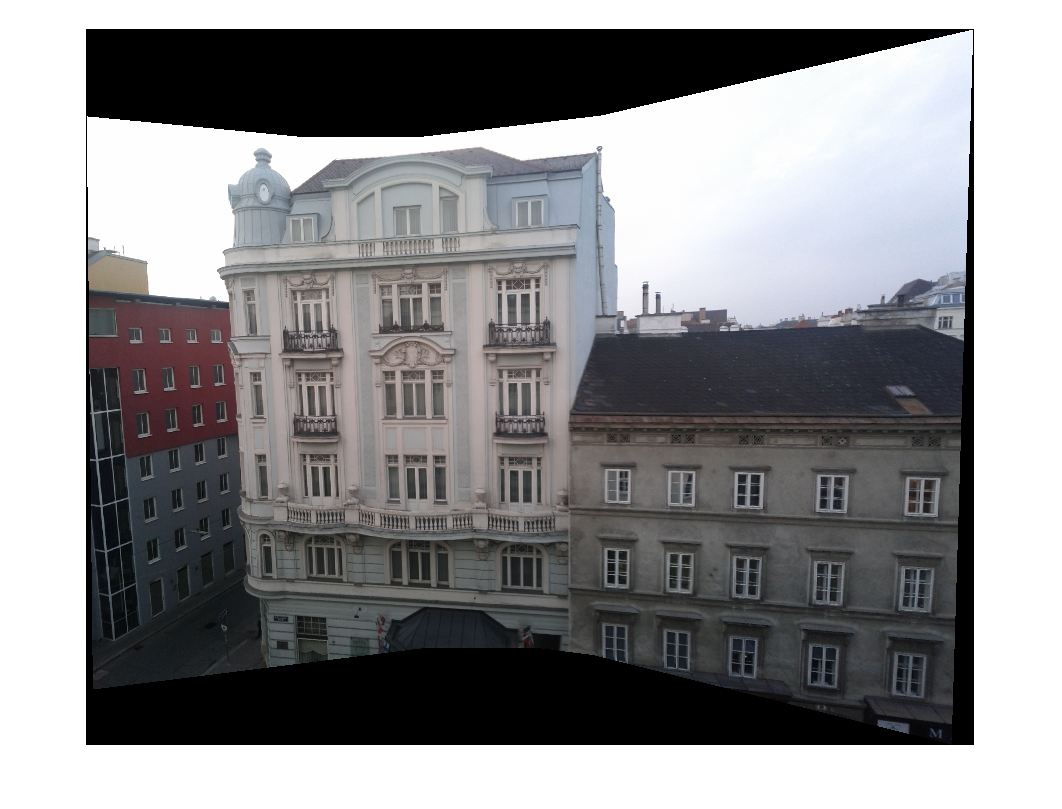
\includegraphics[width=0.45\textwidth]{figures/office_p.png} &
	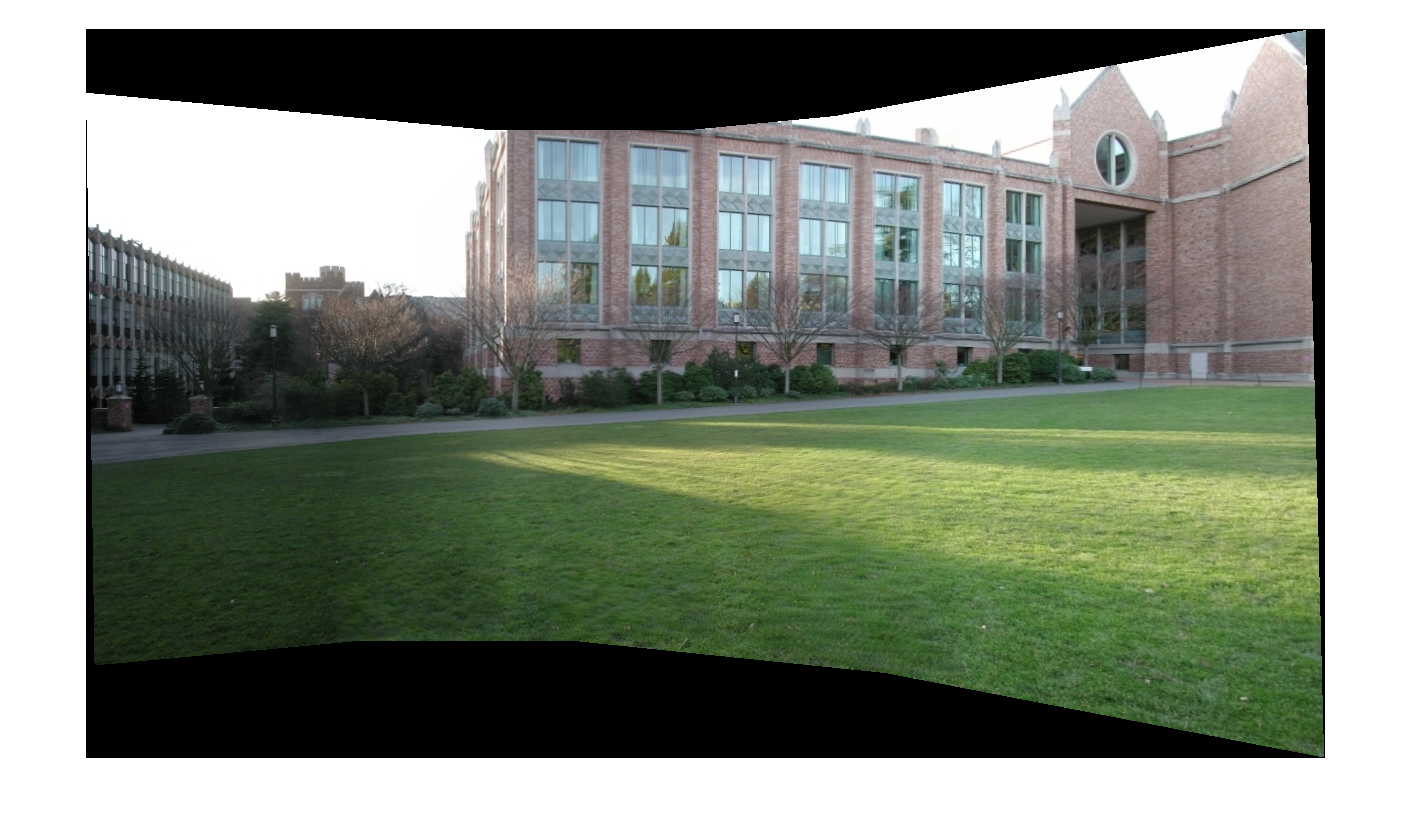
\includegraphics[width=0.45\textwidth]{figures/campus_p.png} \\
	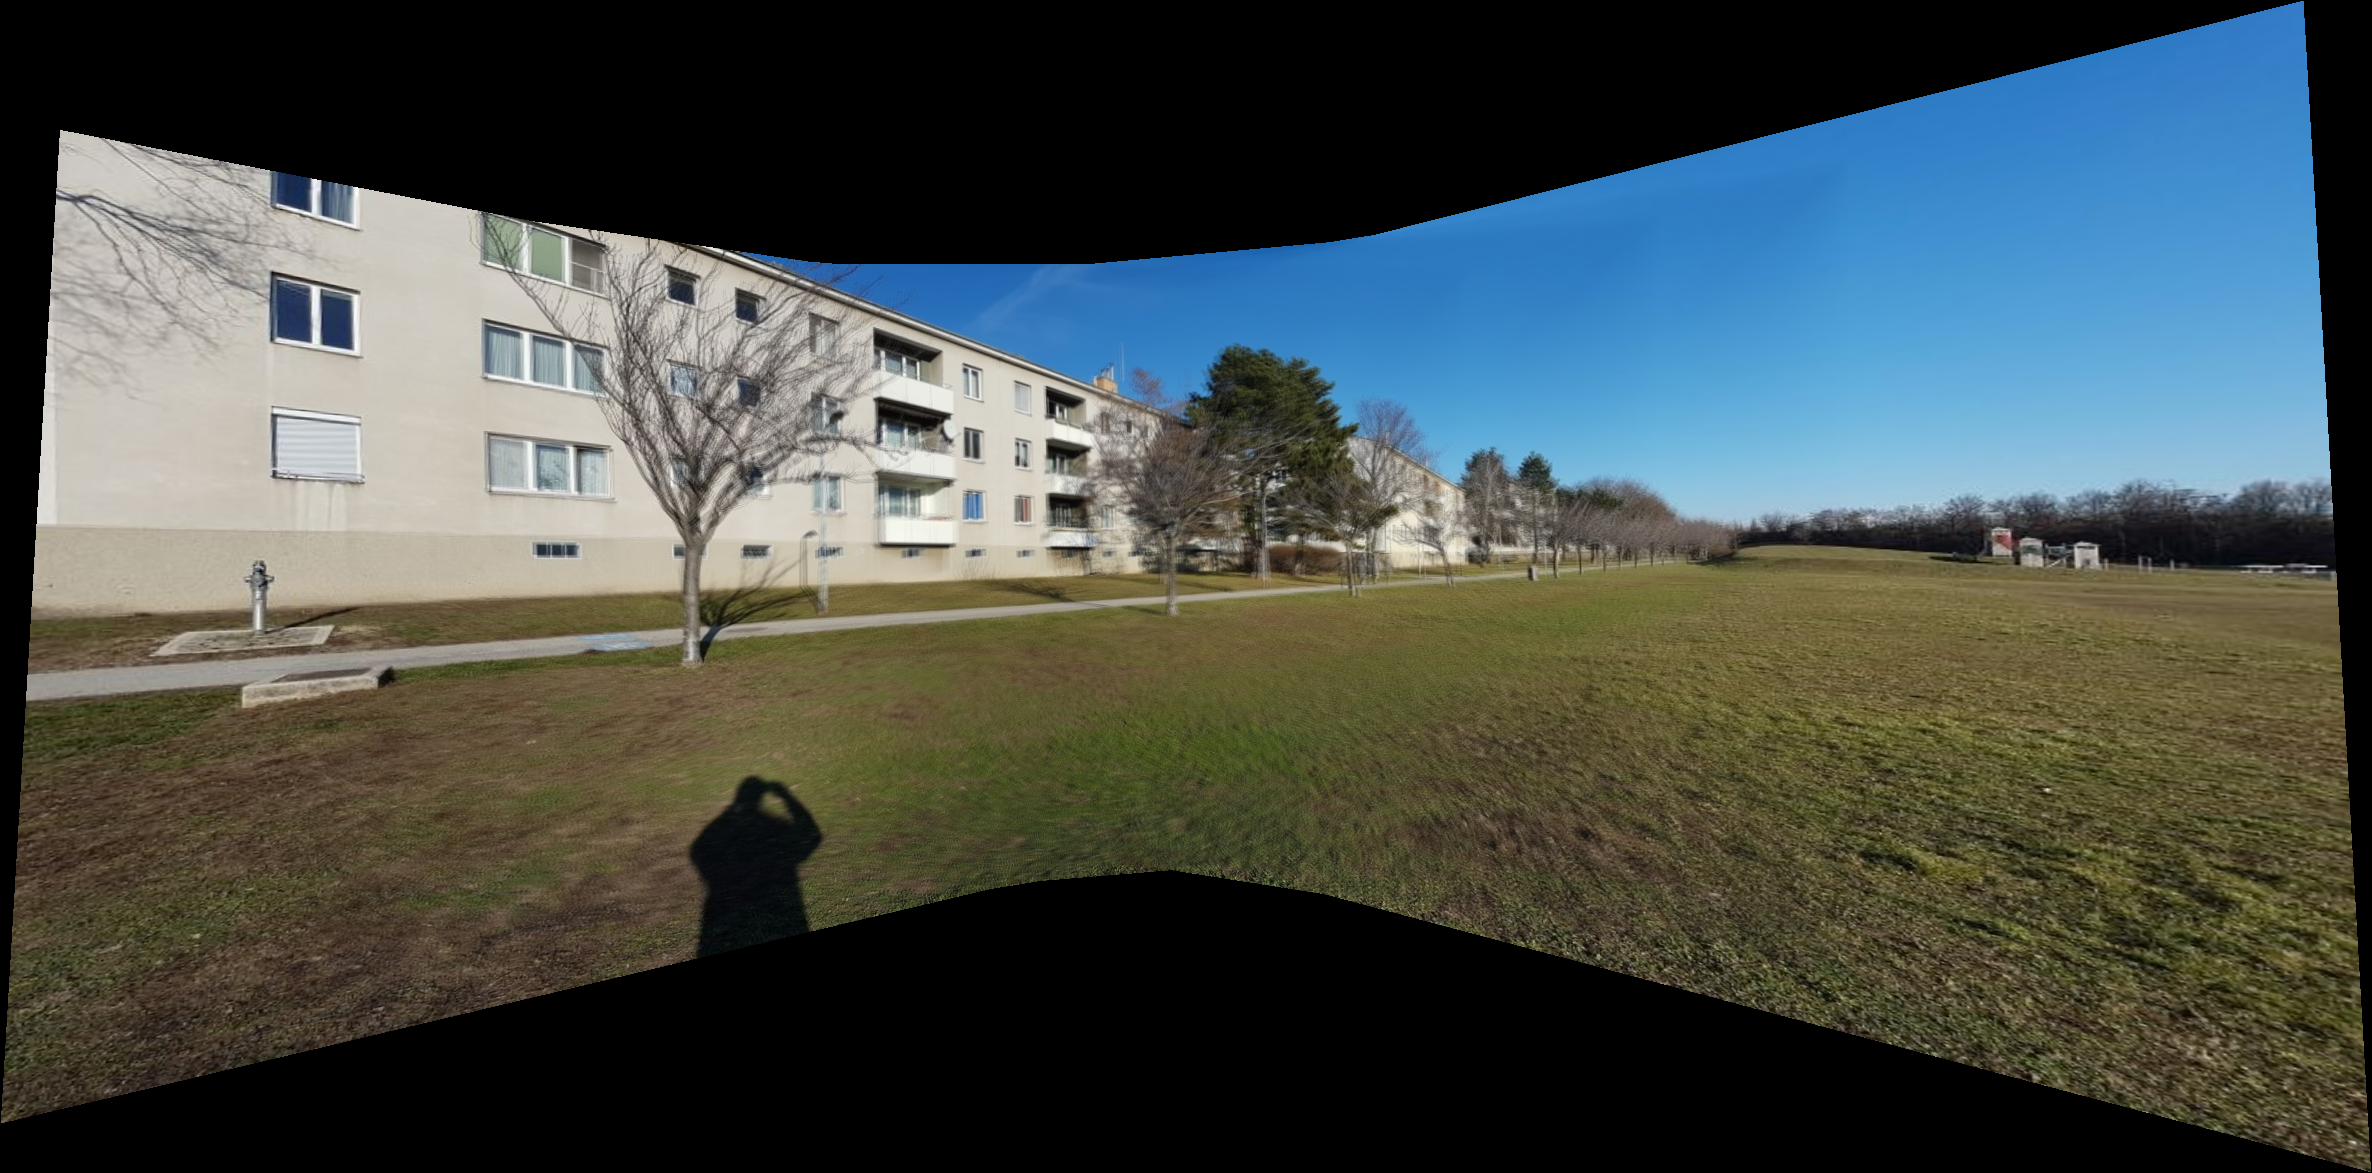
\includegraphics[width=0.45\textwidth]{figures/own_p.png} &
	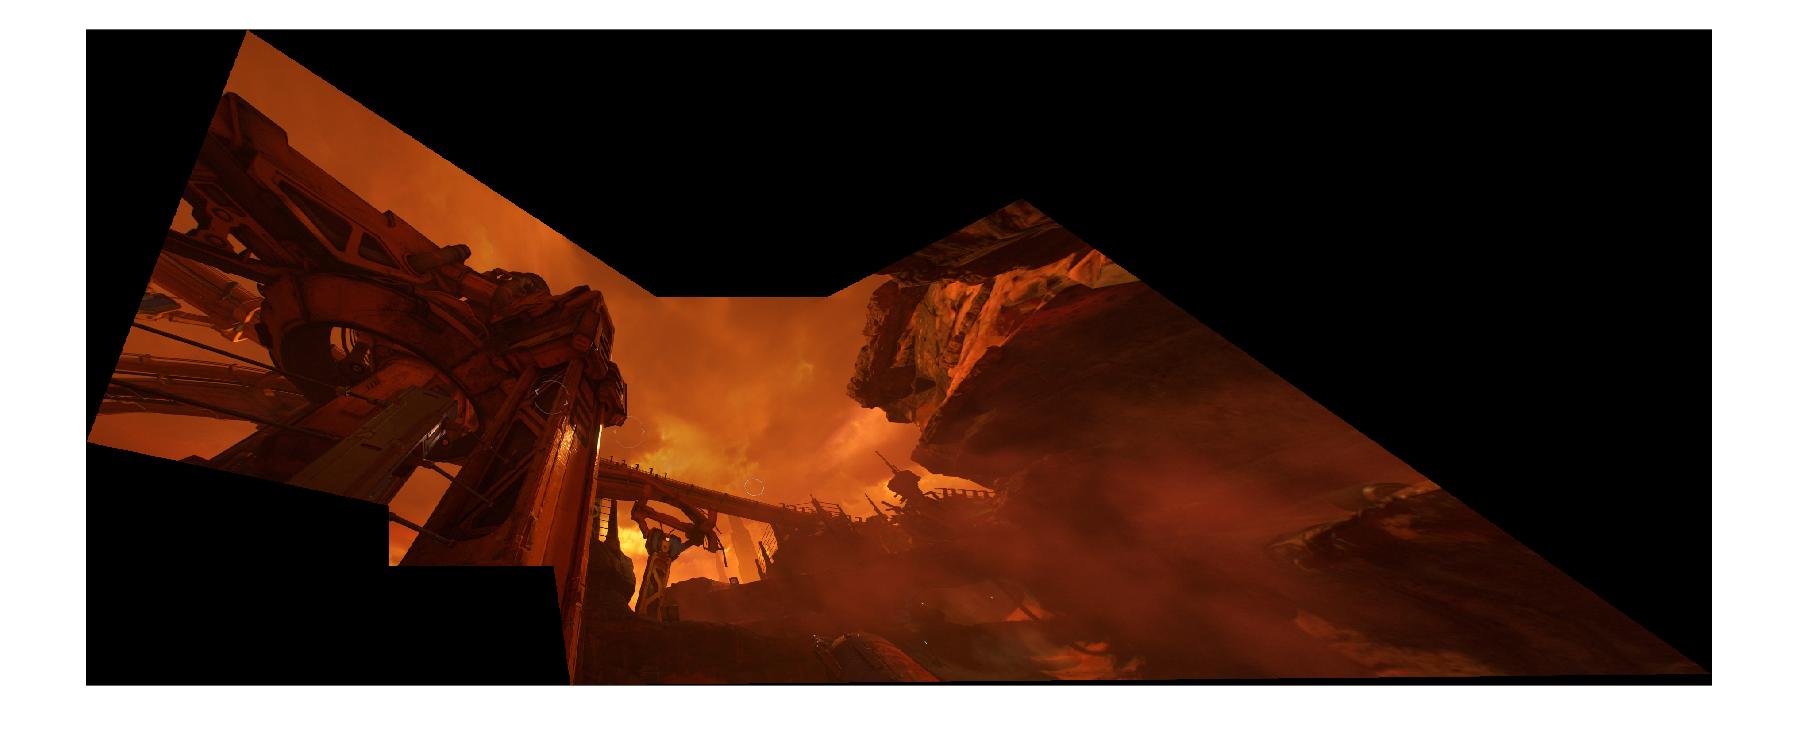
\includegraphics[width=0.45\textwidth]{figures/doom_p.png}

	\end{tabular}
	\caption{Resulting panorama images with feathering.}
	\label{fig:a4:feathering}
\end{figure}


Although the generated panorama images look pretty convincing, upon a closer look one can find different problem spots. These result mainly from imperfect alignment and from image areas of the same location which are different in the separate images. Examples for sources for the latter problem are shadows present in one image, but not in another, or passengers (or other moving objects) that only are captured in some of the images, resulting in ``ghosts''. Both of these problems are most visible in a blended panorama.
In unblended panoramas the most visible artefacts besides the seams are misalignments, which result in jagged areas.
Representatives of each of those problems are shown in Figure~\ref{fig:a4:problems}.

\begin{figure}[h]
	\centering
	\begin{tabular}{cc}
	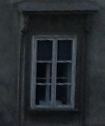
\includegraphics[width=0.25\textwidth]{figures/window_unblended.png} &
	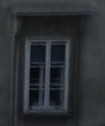
\includegraphics[width=0.25\textwidth]{figures/window_feathered.png} \\
	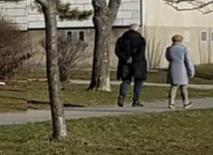
\includegraphics[width=0.25\textwidth]{figures/ghosts_unblended.png} &
	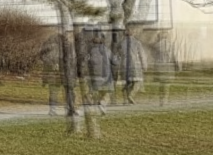
\includegraphics[width=0.25\textwidth]{figures/ghosts_feathered.png} \\
	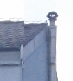
\includegraphics[width=0.20\textwidth]{figures/jagged_unblended.png} &
	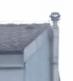
\includegraphics[width=0.20\textwidth]{figures/jagged_feathered.png} \\

	\end{tabular}
	\caption{Problematic areas (left column: unblended, right: feathered). Top: Imperfect alignment, resulting in double-images. Middle: Ghosting of passengers who moved between taking the separate images. Bottom: Jagged connections in the unblended panorama. }
	\label{fig:a4:problems}
\end{figure}
